\chapter{Measurement and monitoring of Muon Trigger System performances}

\section{History and main features of Resistive Plate Chambers}
Before the invention of the RPCs, the first gaseous detectors to operate in the streamer regime were spark and streamer chambers.

\begin{figure}[!t]
\begin{center}
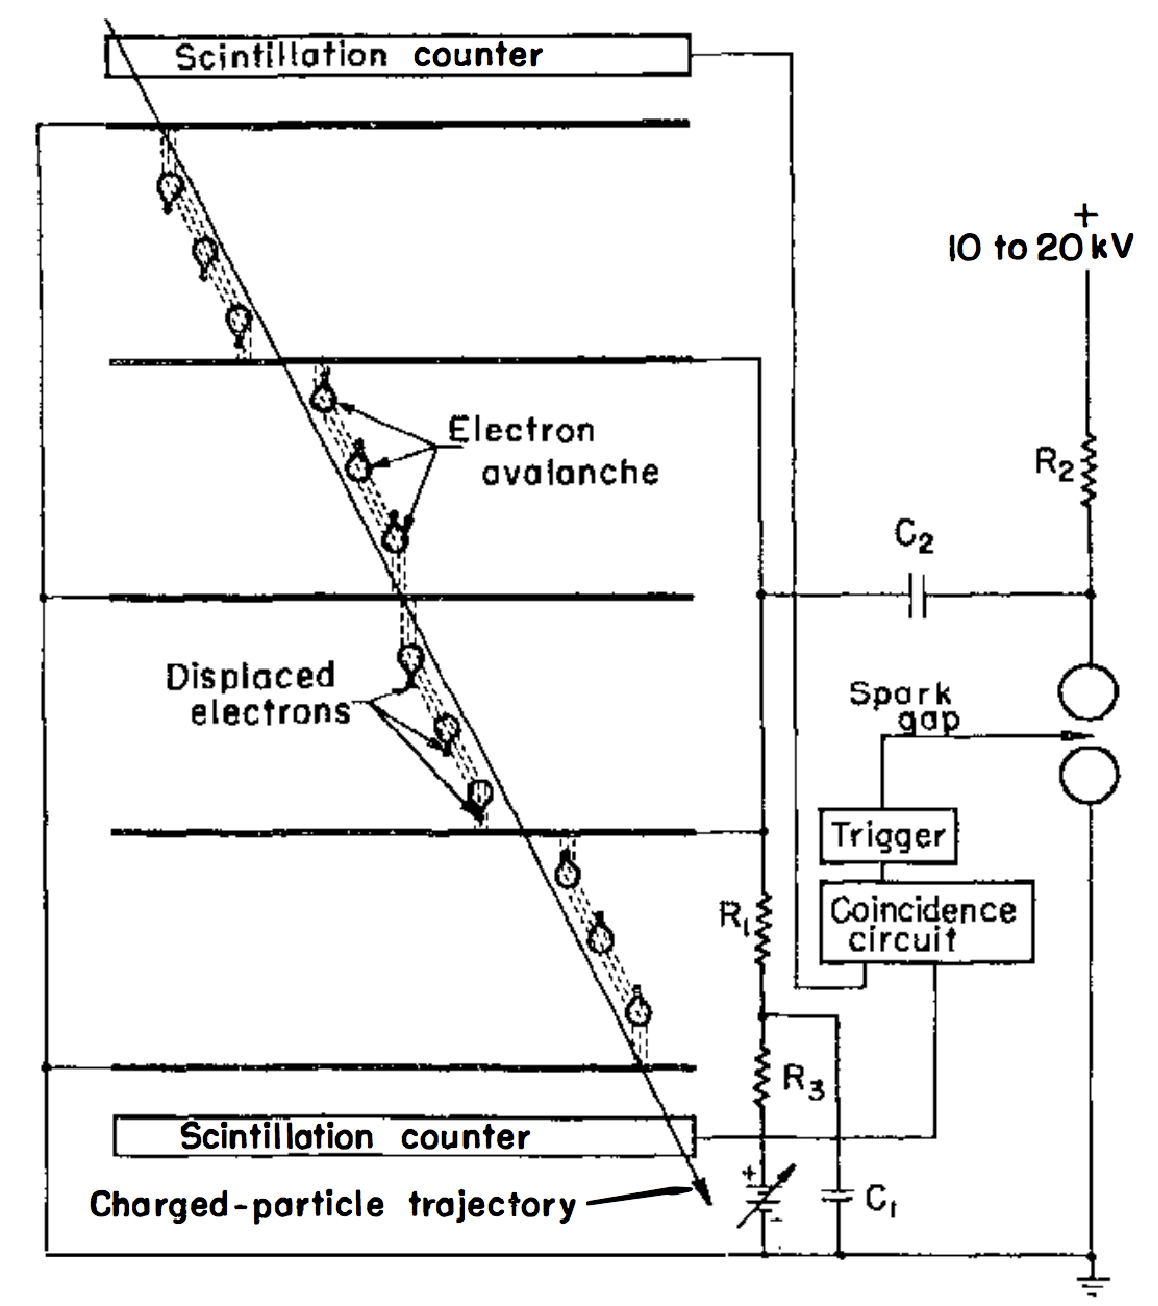
\includegraphics[width=0.95\linewidth]{Chapters/Performance/Figs/spark-chambers.pdf}
\caption{Spark chamber schematic with some details on the external trigger system and coincidence electronics.Extracted from \cite{wenzel:1966}}
\label{fig:SparkChamber}
\end{center}
\end{figure}

Spark chambers (see Fig. \ref{fig:SparkChamber}) are detectors composed of a stack of metal plates put in a sealed box filled with an opportune gaseous mixture \cite{wenzel:1966}.
The metal plates are kept at high voltage, with an electrical field of at least $70 kV/cm$.
An ionizing particle which travels through the detector causes the ionization of the gas, after which the primary electron avalanche develops in $(10^{-8}-10^{-7})s$ and then the secondary ionization and the streamer development happens in $(10^{-10}-10^{-9})s$ after the avalanche \cite{wenzel:1966}.
In the presence of a sufficiently high voltage, the ionized gas can drift causing a trail of sparks that allow one to reveal the ionizing particle path.
% This ionization is typically invisible, but, if enough voltage is applied to the plates, it can cause the drift of the ionized gas which can cause a trail of sparks revealing the ionizing particle path.
The application of the high voltage cannot be permanent, because in this case the creation of a electric arcs would lead to discharge of the whole system.
For this reason an additional detector is needed in order to trigger the application of the high voltage to the plates right during the passing of the ionizing particle.
Typically the high voltage trigger detectors are scintillators. 
In addition whenever a ionizing event happens, the whole interested plates get discharged due to the local conductivity change of the gaseous mixture.
After a full discharge the recovery time is macroscopic, around $10ms$, due the capacitor-like behavior of the plates stack.
In addition, only particles crossing two electrodes caused a spark.

The high dead time due to electrical recovery and the need of an external HV trigger of the spark chambers caused the development of another kind of gaseous detector.
In the past the model for spark growth has prompted several groups \cite{chicovani:1964} to investigate the possibilities of arresting the discharge before the streamers have developed into a spark channel.
The most important consequence of this work is that the isotropic streamer chamber has been invented, in which particle trajectories at all angles to the applied electric field may be recorded.
In addition the streamer chamber allowed one for the recording of more than $30$ tracks at a time.
In this case the electric field is not strong enough to cause an electric arc between the electrodes, but the gradient of the electric field stays strong enough to cause visible streamers around the particle path (see Fig. \ref{fig:Streamer}).
While the HV was still externally triggered by fast detectors, the much lower energy required to develop streamers allowed one to reduce the pulse width to down to $60-100\ ns$.
The typical way of recording a streamer chamber event was by a visible light photo of the streamer cavity.
For this reason the cavity walls required to be transparent.
The streamer mode helped in this task: while the sparks need to reach the electrodes to form, the streamer can be operated with electrodes which are either integrated in the chamber glass walls or external to the glass box.

\begin{figure}[!t]
\begin{center}
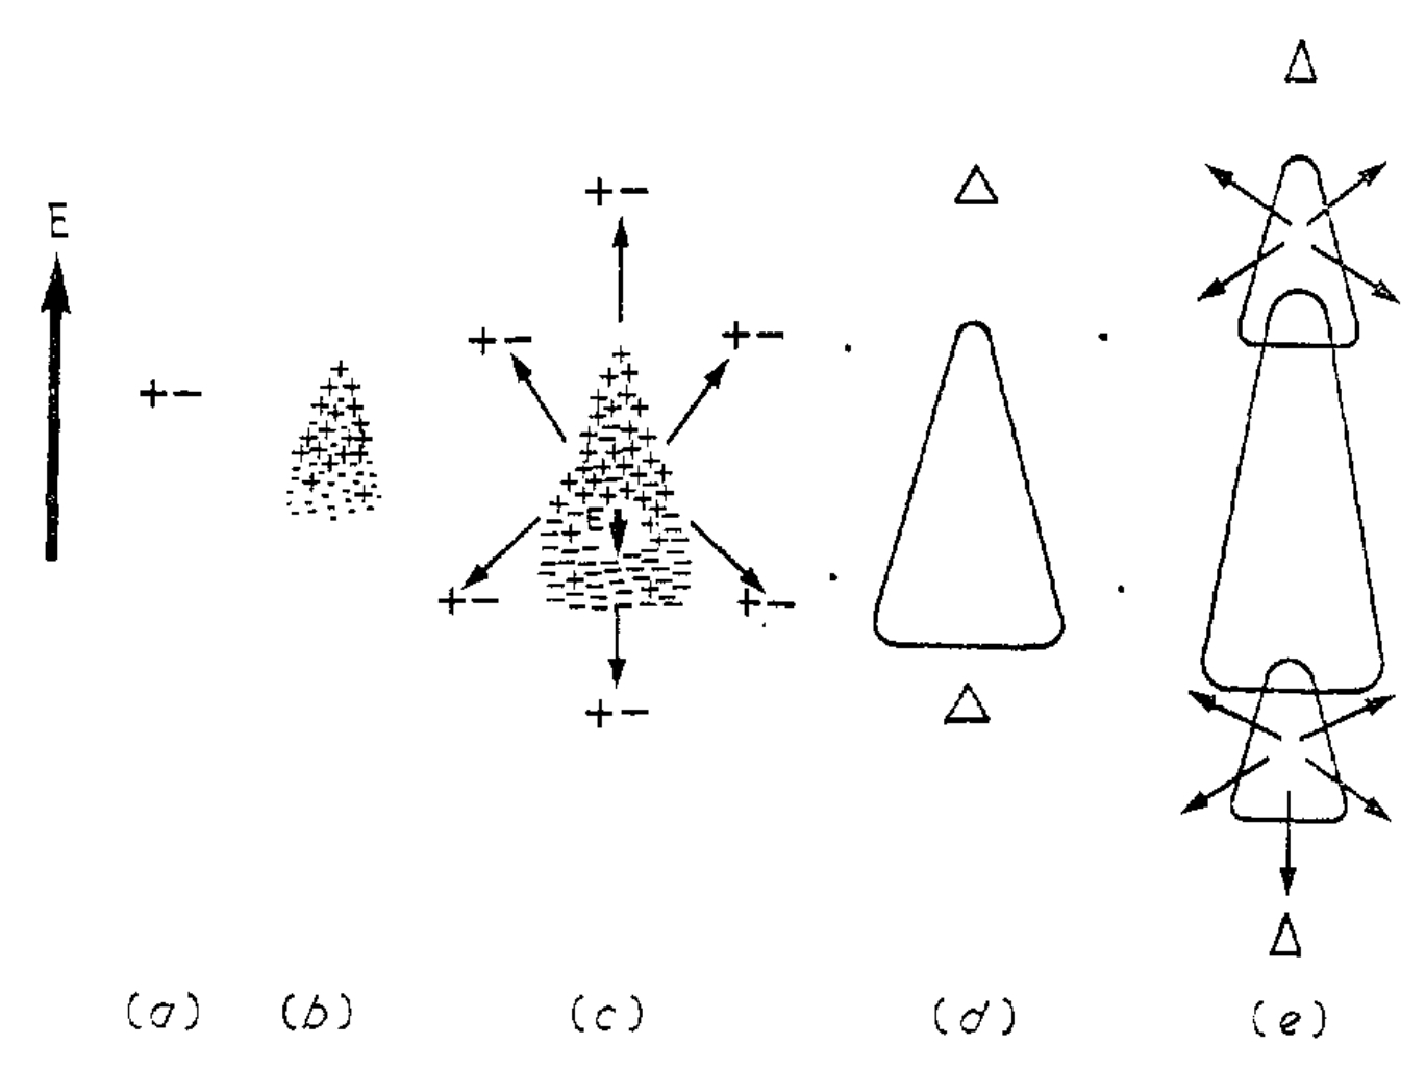
\includegraphics[width=\linewidth]{Chapters/Performance/Figs/streamer.pdf}
\caption{Stages in the growth of a streamer: (a) creation of initial seed electron and positive ion; (b) rapid acceleration of the electrons results in the formation of an avalanche; (c) growth of the avalanche until the internal field compensates the applied field, and recombination causes photons to be emitted which produce more electron-ion pairs; (d) the electrons released at head and tail of the initial avalanche grow into avalanches; (e) continuation of process with merger of avalanches and growth of streamer. From \cite{evans:1969}}
\label{fig:Streamer}
\end{center}
\end{figure}

For the first time the electric field was induced on the gas gap externally, making the gaseous mixture able to generate streamers upon ionization.
Further development of this technology, aimed at reducing the HV pulse length and height, eventually incurred in the avalanche operational mode.
While the streamer is a structure of avalanches which come to saturation and cause a subsequent set of new avalanches, a simple avalanche is a single drop of ionized gas which develops following the electric field gradient.
% At CERN by applying a $300kV$ pulse of $5ns$ length to a gap of $lOcm$, they have been able to arrest the avalanches before growth into streamers.
The discharge size and intensity is obviously reduced from spark mode to streamer mode to avalanche mode.
For this reason the light output diminishes and hence the optical problems become more severe.
At that point the limits of the optical readout (e.g. with a camera) started to appear and caused a further development of such detectors.

\begin{figure}[!t]
\begin{center}
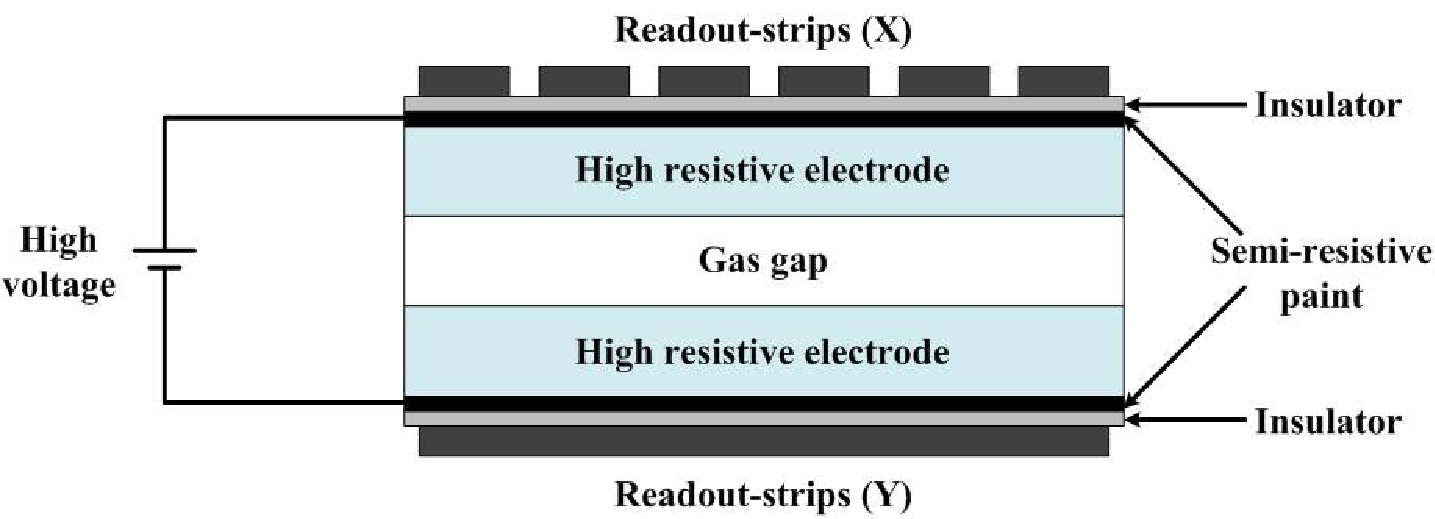
\includegraphics[width=0.8\linewidth]{Chapters/Performance/Figs/RPCside.pdf}
\caption{Schematic representation of an RPC structure from the side.}
\label{fig:RPCside}
\end{center}
\end{figure}

% \section{Resistive Plates Chambers}
% The Resistive Plates Chamber (RPC) detectors were developed taking and improving the best know how achieved for both spark and streamer chambers.
The Resistive Plates Chamber (RPC) detectors were developed by Santonico and Cardarelli \cite{Santonico:1981sc}.
The RPCs are composed of a thin gas gap of some millimeters of thickness and planar resistive electrodes, between which a HV of several kV is applied by means of a graphite coating on the outer face of each electrode.
The signal is picked up inductively by means of copper strips, electrically insulated from the electrodes. 
% The revolutionary idea behind RPCs consists in the use of resistive electrodes to provide the electric field.
The use of a resistive electrode ensures that the reduction of the electric potential between the electrodes is local, meaning that the detection happens without a complete discharge of the electrodes.
Moreover, the local nature of the discharge makes RPC an intrinsically position-sensitive detector.
% This aspect of the RPCs working mode allowed to drop the requirements for an external array of detectors which served as a trigger for the HV pulse, since the HV could be provided constantly and dynamically re-established in the case of a local discharge.
% This development of the gaseous detectors technology brought back this approach on providing big coverage and cheap detectors capable of sustaining high particle rates providing fast response time ($ns$) with good spatial resolution (millimeter) and high efficiency.
The RPCs are relatively cheap detectors with a fast response time (of the order of $ns$) and good spatial resolution (slightly better than $1\ cm$) that can therefore cover large surfaces and sustain high particle rates.
RPCs are currently adopted, mainly as muon detectors, by ALICE, ATLAS and CMS at the LHC and many other particle physics experiments around the world.

% \section{Main features of RPC detectors}
RPC detectors are made of several layers of different materials.
First of all the gas gap is the innermost part of the detector and contains a gas mixture which will be discussed later.
% The gas gap is surrounded by the high resistivity electrodes which are the HV providers and thanks to the high resistivity are able to spatially limit the discharge.
Electrodes resistivity is of the order of $10^{9}-10^{10}\ \Omega \cdot cm$.
The roughness of the electrodes must be as low as possible to limit the peak discharge around surface anisotropies.


\begin{figure}[!t]
\begin{center}
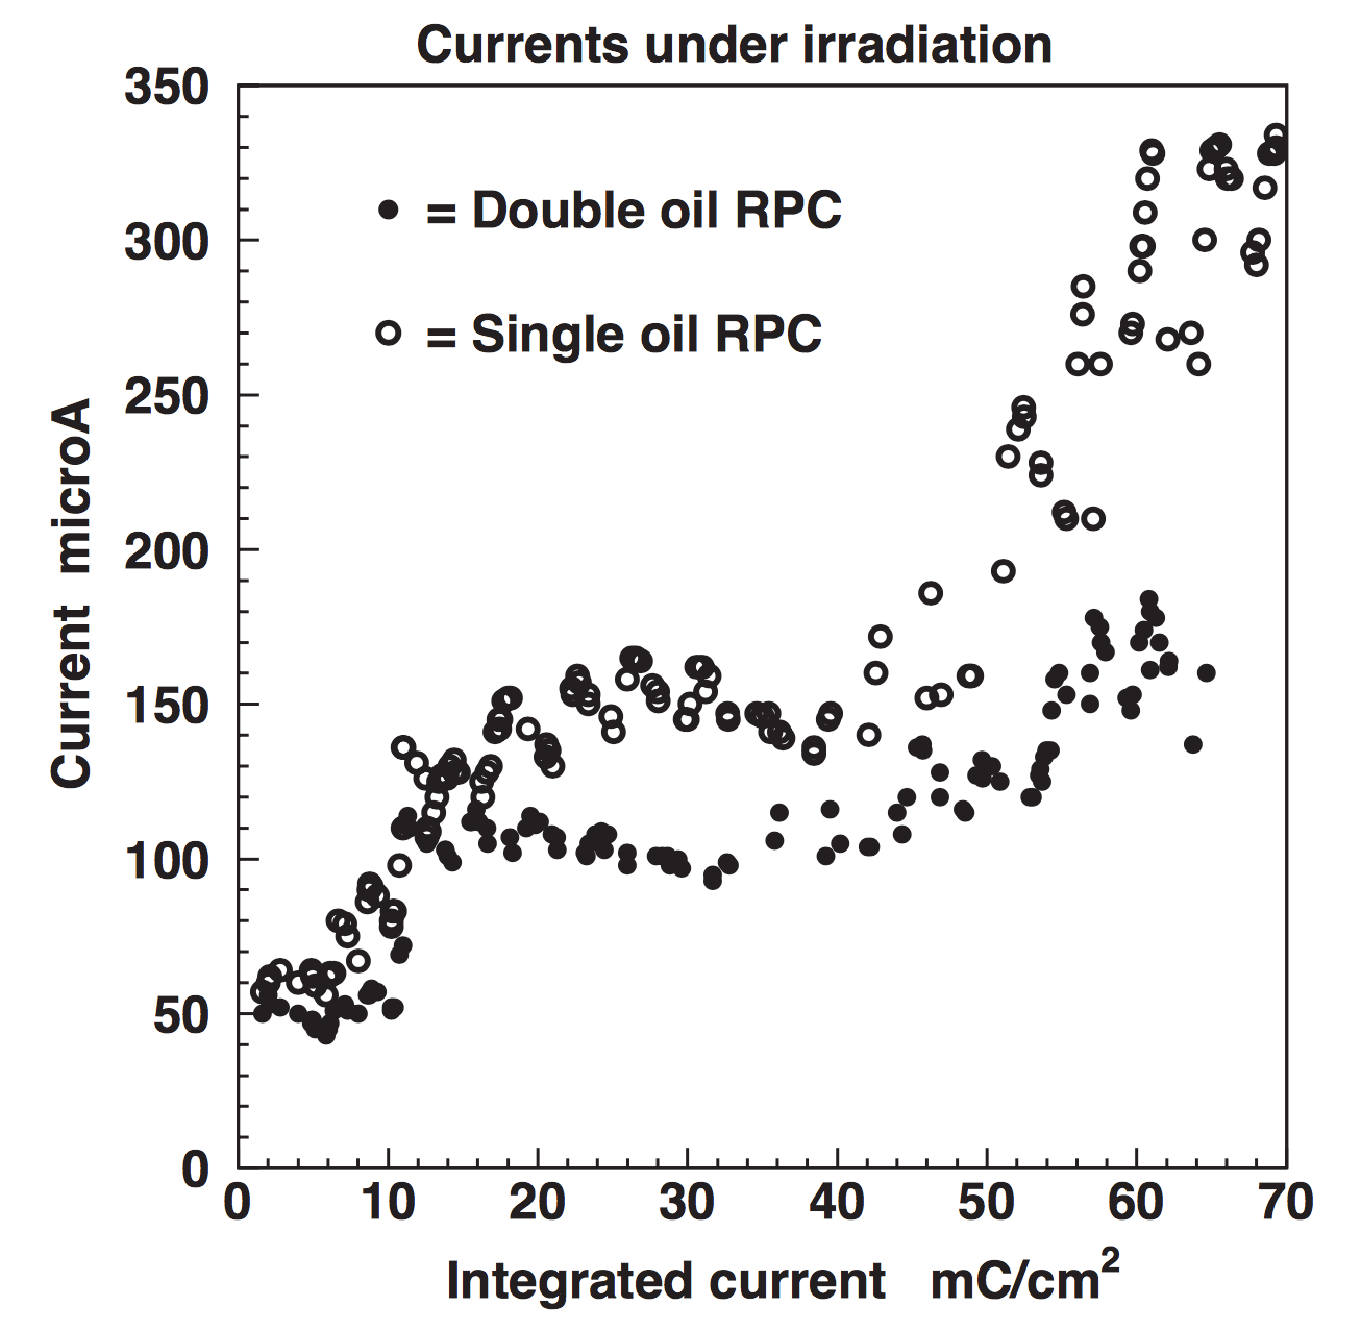
\includegraphics[width=0.47\linewidth]{Chapters/Performance/Figs/oil_irradiation.pdf}
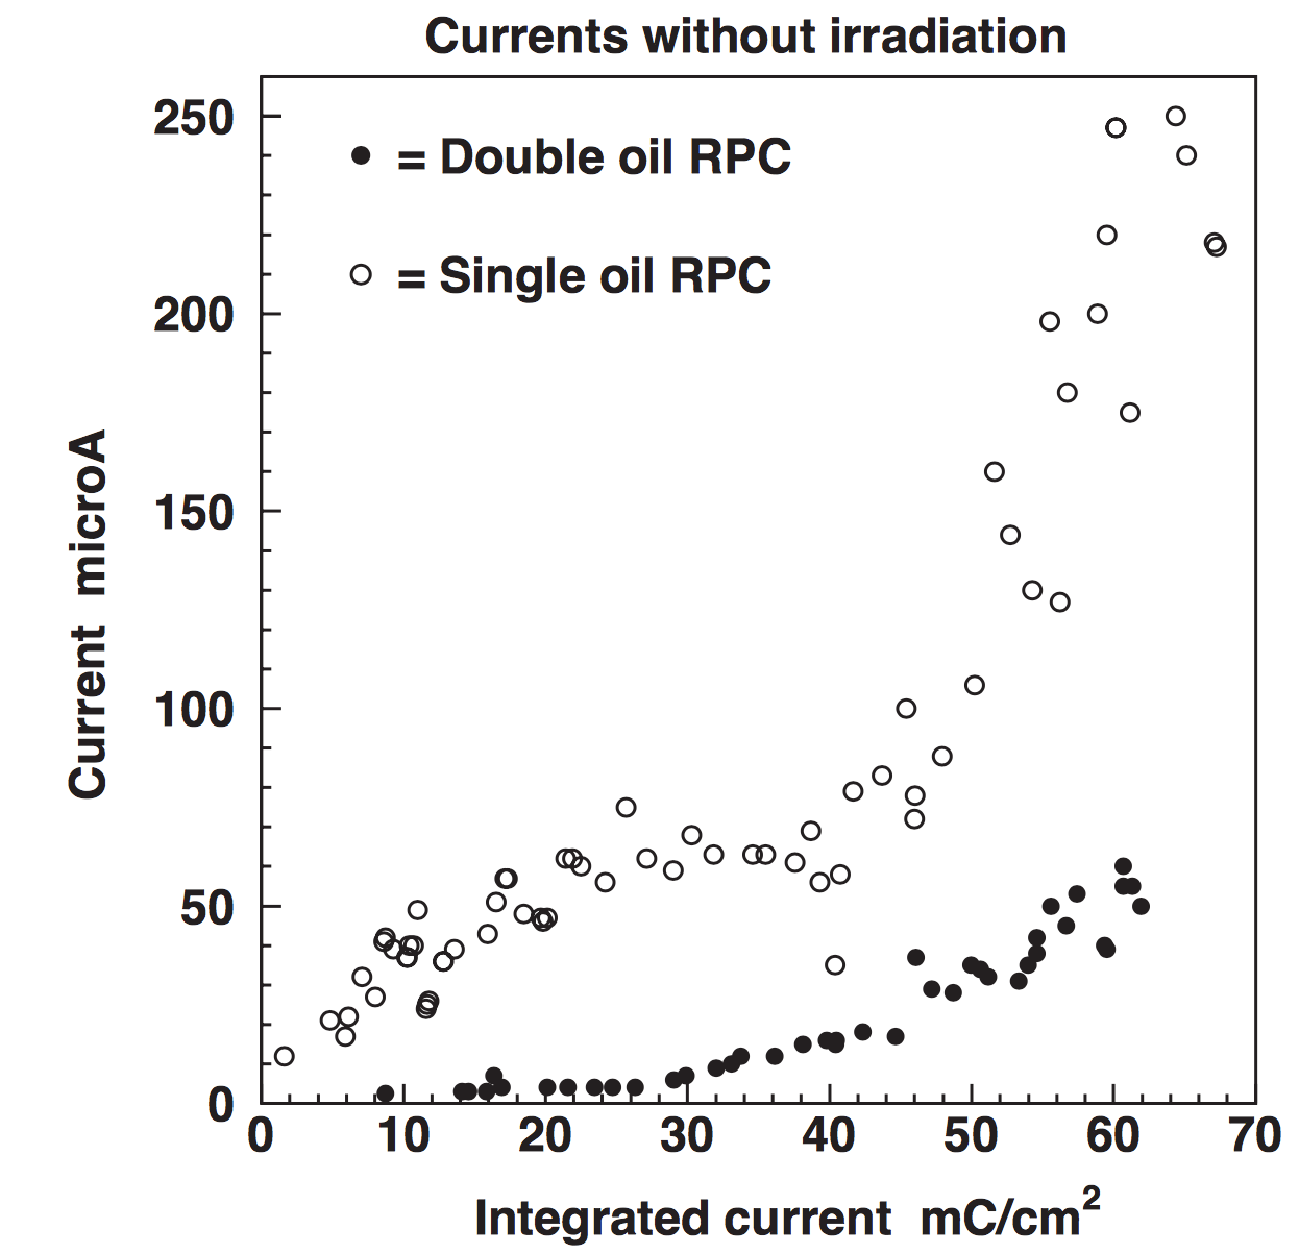
\includegraphics[width=0.47\linewidth]{Chapters/Performance/Figs/oil_no_irradiation.pdf}
\caption{Current trend over time for single side oil coated and double oil coated RPCs. From \cite{aliceRPC:2004}.}
\label{fig:RPCoil}
\end{center}
\end{figure}

For this reason the resistive electrodes are frequently coated with oils in order to improve the smoothness of the inner surface and to preserve the resistivity (see Fig. \ref{fig:RPCoil}).
Right outside the resistive electrodes an insulation layer made of plastic material is provided, in order to electrically decouple the internal electrodes and the pick-up strips.
The readout pads or strips are installed outside the insulation layer.
The edge of the chamber is sealed  by means of plastic material walls and is equipped with pipes for the flow of the gaseous mixture.

The gaseous mixture of a RPC is not standard and each implementation can differ from any other one.
However, some basic ingredients can be identified:
\begin{itemize}
\item Donor gas: ($e.g.$ $Ar$) it is the gas that should be ionized by the ionizing particle and which provides amplification of the deposited charge via secondary ionisation;
\item X-ray quencher: ($e.g.$ $iC_4H_{10}$) it is a gas that has an high cross section for x-rays and high energy photons. This is needed in order to absorb recombination photons that can cause a degeneration in streamer;
\item Charge quencher: ($e.g.$ $SF_6$) it is a gas that provides high electro-negativity in order to limit the transversal development of the avalanche and reduce the probability of a streamer degeneration.
\end{itemize}

Depending on whether the RPC is chosen to operate in avalanche or streamer mode (Fig. \ref{fig:Streamer}) the gas mixture should be modified.
For example a streamer mixture is mainly composed of Argon, while in avalanche mixtures this is replaced by a gas which, along with acting as a donor, has also quenching properties ($e.g.\ C_2H_2F_4$).
% The chosen mixture is always engineered for one of the two working modes and cannot be used in the other one.

Several aspects, such as the gas mixture composition, enter the definition of an RPC HV working point.
Typically this voltage is chosen by performing an efficiency versus voltage scan of a specific RPC, and might differ from one RPC to another.
Apart from the detection efficiency, other aspects are important and should be considered when selecting the working point of an RPC.
A dependence between the supplied HV and the distribution of the cluster sizes (namely the number of adjacent strips fired by a single particle) has been observed, hence while the efficiency arises when raising the HV, the spatial resolution might be affected.
Another aspect related to the HV value is the signal amplitude and the total charge deposed in the gas gap by a ionizing particle.
The choice  of the RPC gas mixture and HV is strictly connected to the characteristics of the front-end electronics (FEE) used for the read-out. 
The signal amplitude required is defined by the minimum threshold that can be set in the FEE, which in turn depends on the FEE’s noise level. 
In some applications, the usage of FEE cards with an amplification stage allows for low-gain operation \cite{Marchisone:2017bcb}.
% In the end the working point choice is related to the kind of read-out electronics, since it is defined as the high voltage at which the chamber can provide enough detection efficiency for a specific application.

% The readout of the chamber is performed via a front-end electronics which is connected to the readout electrodes.
% The readout sensitivity has to be tuned based on the signal amplitude of the chamber.
% % At this point two roads are possible.
% A signal multiplication has to be performed in order to be able to detect the ionizing particle.
% A signal multiplication has to be performed in order to make detectable the ionizing particle.
% The multiplication can be either performed by saturating the avalanche inside the gas gap, using the ionization process, or by keeping a low avalanche saturation in the gas gap, using an amplified electronics as readout.
% In this second case a lower voltage in the cathode is required.
% In the second case the high voltage can be lowered with respect to the first case, in which the amplification in the gas gap in fed by the HV supply.


\section{Ageing effects in RPC detectors}
Like other gaseous detectors, the gas gap of the RPCs can undergo during long-term operation reversible and irreversible performance degradation.

The most important source of performance degradation is the amount of charge generated in the gas gap during irradiation at nominal voltage.
% In fact the charge generated in the gas gap is deposed either on the resistive electrodes or can induce the generation of chemical compounds out of the gas mixture components.
The avalanche (or streamer) process can directly harm the electrodes or, more frequently, induce the generation of chemical compounds other than the gas mixture components.
These compounds might form deposits on the inner surfaces of the gas gap, creating peaks which can affect the chamber noisiness, as well as they can chemically attack the surfaces.
Both these situations can cause an increase of the noise rate of the chambers.
An high noise rate causes a local inefficiency of the detector due to the recovery time after a discharge.
% Even if one would like to avoid as much as possible these irreversible alterations, they are physiological of the RPC detectors used in such high irradiation situations.
These processes can be mitigated by special measures.
% For example the ALICE RPCs, and in general any other implementation of such detectors in modern experiments, are fed with a constant flux of gas in order to clean the gas from unwanted chemical compounds.
% In addition to the filtering of the gaseous mixture and the constant replacement of part of that, the gaseous mixture is humidified.
Besides the already mentioned oiling of the inner surface  of the electrodes, another common measure is the usage of a humid gas mixture.
Indeed, one of the risks for bakelite-made RPCs is the mechanical deformations and the resistivity variations caused by the drying of bakelite layers.
The humidification of the gaseous mixture allows one to constantly hydrate the inner surface of the bakelite electrodes, keeping the original gas gaps shape and avoiding changes of the bakelite resistivity (see Fig. \ref{fig:drywet}).

\begin{figure}[!t]
\begin{center}
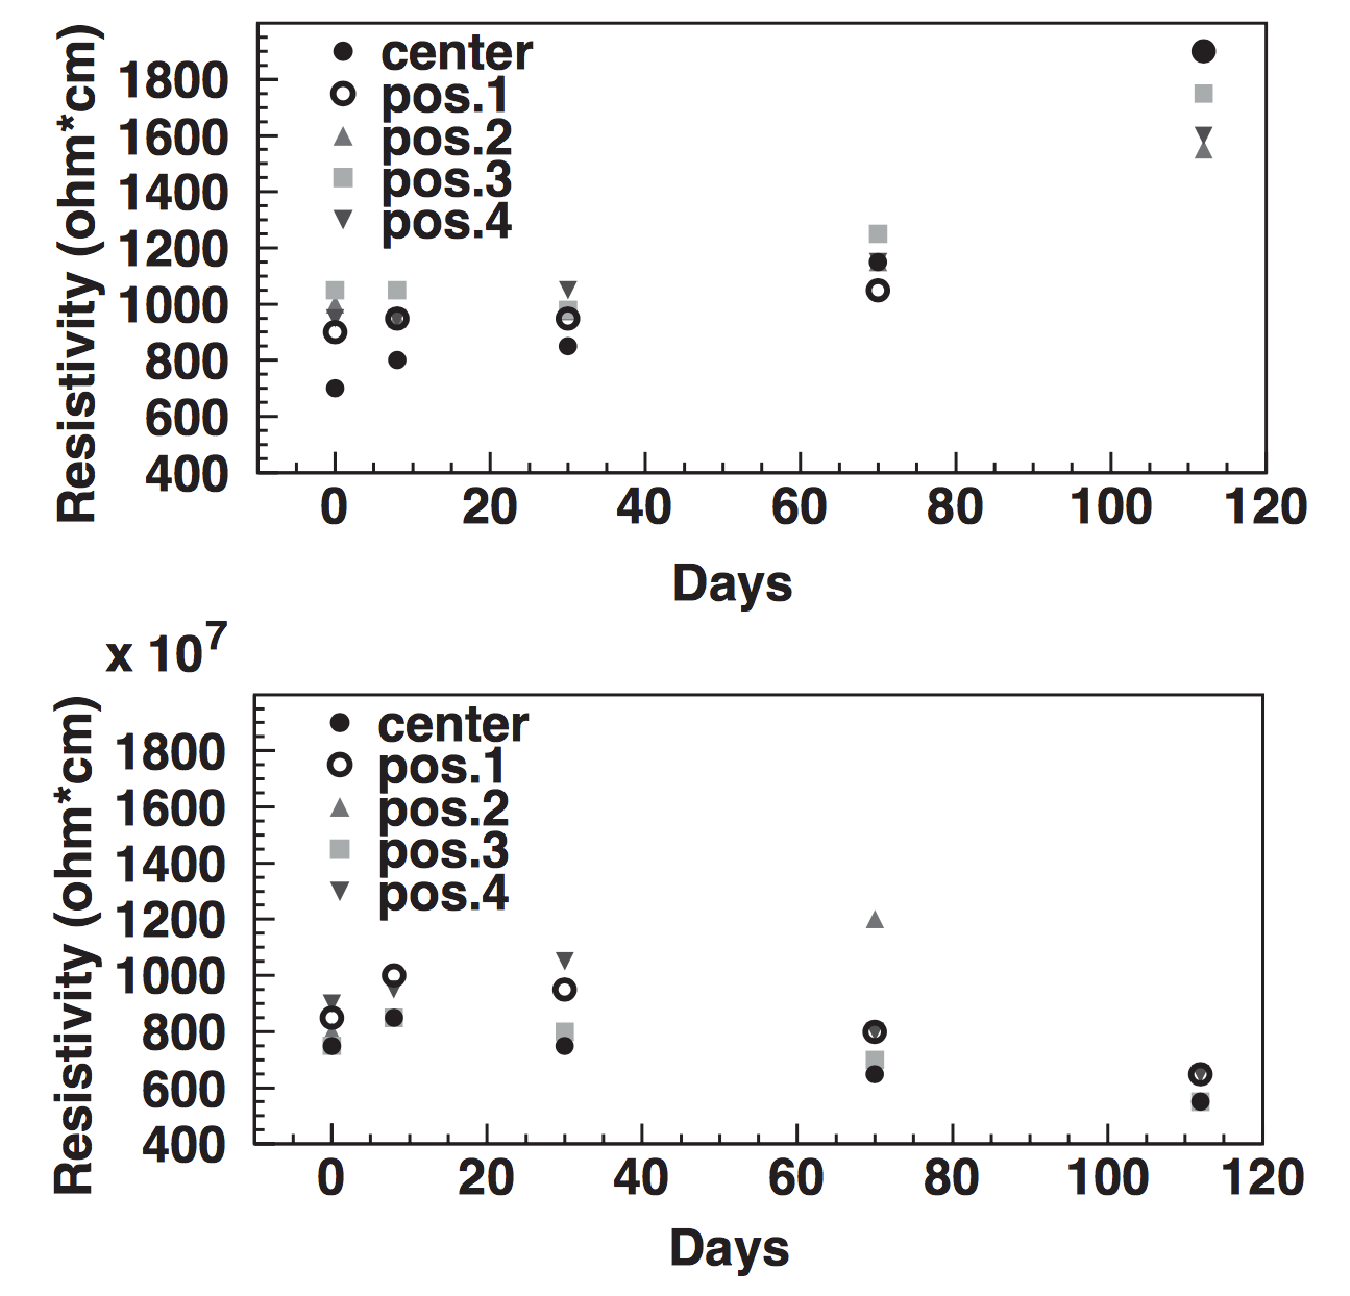
\includegraphics[width=0.95\linewidth]{Chapters/Performance/Figs/dry_vs_wet.pdf}
\caption{Resistivity trend over time for prototype ALICE RPCs. In the top panel a chamber provided with dry gas mixture is shown, while in the bottom panel the gas mixture is humidified. Different marker styles correspond to different testing positions. From \cite{aliceRPC:2004}.}
\label{fig:drywet}
\end{center}
\end{figure}

% The most important source of performance degradation is the amount of charge generated in the gas gap during irradiation at nominal voltage.
% In fact the charge generated in the gas gap is deposed either on the resistive electrodes or can induce the generation of chemical compounds out of the gas mixture components.
% These compounds might depose on the inner surfaces of the gas gap, creating peaks which can affect the chamber noisiness, as well as they can chemically attack the surfaces.
% Both these situations can cause an increase of the noise rate of the chambers.
% An high noise rate causes a local inefficiency of the detector due to the recovery time after a discharge.


% For this reason the monitoring of the chambers has to be performed in order to detect as soon as possible the most altered chambers and to proceed with their replacement with spare ones.
% As found at the GIF tests the ALICE muon trigger RPCs are performing well enough at least up to a total deposed ionization charge of $50mC/cm^2$.
% The integrated charge is for this reason the main aging indicator for our RPCs.
% If the integrated charge crosses the limit the chamber behavior might become unstable.
% For this reason RPCs getting closer to the tests limit have to be replaced at the first possible occasion.

The “age” of a RPC detector is frequently quantified by means of the integrated charge ($mC/cm^2$). 
Detectors are ageing tested at high-intensity photon sources to simulate the effect of long-term operation.

% In addition to the evaluation of the integrated charge some others aging indicators can be spotted.
% Even if the RPCs discharge is spatially limited by their resistivity, a localized discharge causes a temporary inefficiency due to the fact that the voltage should be reestablished.
% The dark current is an interesting parameter, since it is usually related to the smoothness of the inner surfaces.
% In fact having a coarse and spiked inner surface is not ideal: the irregularities might enhance the spikes effect, hence the frequency of dielectric breakdown.
% This situation can lead to a local efficiency drop, more or less important depending on the ratio between the breakdown frequency and the HV recovery time.
% In case of a worsening of the inner surfaces smoothness one might expect an increase over time of the dark current.

% Another parameter, related to similar considerations, is the dark rate.
% All the considerations performed for the dark current are valid also for the dark rate.

Along with the efficiency of the detector, two among the most important parameters to be monitored to assess ageing are the dark current and the dark rate, $i.e.$ the current and counting rate of the detector at nominal high voltage in absence of beam.
These quantities are expected to be sensitive to the quality of the inner surface of the electrodes, as the presence of spikes or dips may enhance electron extraction from the cathode and consequent development of an avalanche or streamer.
Moreover, the dark current is sensitive to ohmic effects due to non-perfect insulation of the HV plate from the rest of the system.

% The three observables presented up to this point are studied trough the analysis of their values plotted over time.
% Additional studies and observations may be performed using meaningful correlation plots.
% Such plots, which are provided out of the box by the new MTR analysis framework, allow for the correlation of two of the stored variables.
% For example the correlation plot between the net current and the rate observed at nominal HV during collisions can be fitted with a sloped line.
% The angular parameter of the fit is an evaluation of the deposed charge per crossing ionizing particle.
% A distribution of such parameter for the whole set of 72 RPCs might help spotting the outliers, namely the RPCs for which the charge deposed for a given ionizing particle is higher.
% The detectors showing an higher charge per ionizing particle have to be strictly monitored, since their integrated charge will increase faster with respect to the normal ones.

% The framework allows to produce distributions of the recorded values with respect to the beam conditions, hence relationships between the colliding systems and their energy and the RPCs behavior may be studied.

In the second part of this chapter, the framework developed for the monitoring of the parameters mentioned above for the RPCs of the ALICE muon trigger will be described.

\section{The ALICE muon trigger RPCs}
The ALICE muon trigger system is made of four layers (MT11, MT12, MT21 and MT22) arranged in two stations spaced of $1.2m$, as shown in figure \ref{fig:ALICEmuon}.
Each layer is divided in two half-planes, inside LHC ring and outside LHC ring (INSIDE and OUTSIDE in the following).
Each of the four layers is composed of 18 RPCs.
The chambers of the first two stations are slightly smaller than the ones of the third and fourth in order to cover the same pseudorapidity range.
Three shapes of RPC are installed and correspond to long, short and cut shapes.
The short and cut shapes are intended to leave the necessary clearance for the beam pipe.
The muon trigger RPCs are made of $2mm$ wide gas gaps with $2mm$ thick bakelite resistive electrodes and polyammide insulation layers.
The readout strips are copper made and their pitch can vary among three values: $1cm$, $2cm$ or $4cm$.
All the RPCs are equipped with one set of readout strips per side.
The strips of each side of the RPCs are reciprocally orthogonal.
The vertical (horizontal) strips, providing $x$ ($y$) hits, are called non-bending (bending) in relation to the dipole action on charged particles paths.
The currently installed front-end electronics is called ADULT and is not amplified \cite{Dupieux:2003bw}.
71 RPCs are equipped with this electronics, while one RPC is equipped with a prototype of the FEERIC electronics \cite{Marchisone:2017bcb} that provides an integrated amplification stage.
The ALICE muon trigger RPCs (and the ADULT electronics) were initially developed for streamer mode operation \cite{Arnaldi:2000ub}. 
Later on, a second operation mode (“maxi-avalanche”) was developed \cite{Arnaldi:2006ii}, where the signal amplitude is smaller than in streamer mode, but still compatible with the minimum threshold ($\approx7\ mV$) that can be set in ADULT. 
The beam test performed in maxi-avalanche mode showed a rate capability ($i.e.$ the maximum irradiation rate that can be reached without efficiency degradation due to the local voltage drop) of about $80\ Hz/cm^2$. 
Moreover, prototypes were ageing-tested at the CERN Gamma Irradiation Facility up to an integrated charge of about $50\ mC/cm^2$.
The gas mixture corresponding to such an operation mode is:
\begin{itemize}
    \item $89.7\%$ Tetrafluoroethane ($C_2H_2F_4$);
    \item $10.0\%$ iso-Buthane ($iC_4H_{10}$);
    \item $0.3\%$ Sulfum esafluoride ($SF_6$).
\end{itemize}
As will be discussed in Chapter 4, the ALICE experiment will undergo a major upgrade before the LHC RUN3 (expected to start in 2021), where the instantaneous luminosity in Pb-Pb collisions will increase by almost one order of magnitude. 
In light of this, the FEERIC electronics was developed. 
The goal is to lower the HV and operate the detectors in pure avalanche mode, transferring the gain from the gas to the electronics, decreasing the deposited charge per hit by about a factor $\approx4$ and hence improving the rate capability and reducing the impact of ageing effects. 
Since the beginning of the LHC RUN2 (2015) one RPC is equipped with FEERIC, in order to test in real life the expected performance improvement.
% This development has been pursued to improve the performances and the rate capability of the current detectors.
% The current read-out board is called ADULT and was developed to work in streamer operation mode, thanks to a dual threshold discriminator with modifiable thresholds.
% Even if ADULT performed well, the streamer mode was never used in the muon trigger RPCs.
% Thanks to the modifiable thresholds ADULT operated in avalanche mode effectively for the last 10 years.
% However, the signal dynamics of an avalanche is much smaller than that of a streamer, since only in the latter in-gas multiplication is possible.
% Based on these two arguments, a new single threshold electronically amplified electronic read-out board has been developed.
% This new board is called FEERIC and is specialized in reading signals coming from avalanche operation mode and adopts a mosfet amplification stage.
% The effects of an amplified electronics are various.
% First of all the required charge dynamics in the gas gap is much lower with respect to that required by an non-amplified read-out.
% The free charge of the signal is in fact collected by the electrodes and amplified out of the gap.
% Lowering of the charge per hit allows to have smaller dead times since restoring the original HV requires less energy.
% Requiring a lower charge has the side effect of allowing a reduction of the operating HV, which leads to a even faster recovery time.
% The drawback of the adoption of an amplified electronics is that small noise signals, which a non-amplified electronics does not detect, might become observable and detected.
% One RPC currently part of the ALICE muon trigger is equipped with FEERIC since 2015, in order to offer an insight of the improved performances.
% FEERIC will equip the whole muon trigger system from the LHC RUN3 (2021 onward).
The working point of the ADULT-equipped RPCs is about $10200\ V$, while for the FEERIC-equipped RPC the working point is about $9500\ V$, $i.e.$ $700\ V$ lower than with ADULT.
During the operation the variation of the atmospheric temperature (T) and pressure (P) results in a variation of the efficiency.
This effect can be corrected for by dynamically adjusting the high voltage according to the formula:
% The HV tuning formula is:

\begin{equation}
\label{eq:HVcorrection}
HV = HV_{nom}\cdot \frac{T_0}{T} \cdot \frac{P}{P_0}
\end{equation}

where $HV_{nom}$ is the working point quoted above, $p_0 = 970\ mbar$ and $T_0 = 293.15\ K$.

\begin{figure}[!t]
\begin{center}
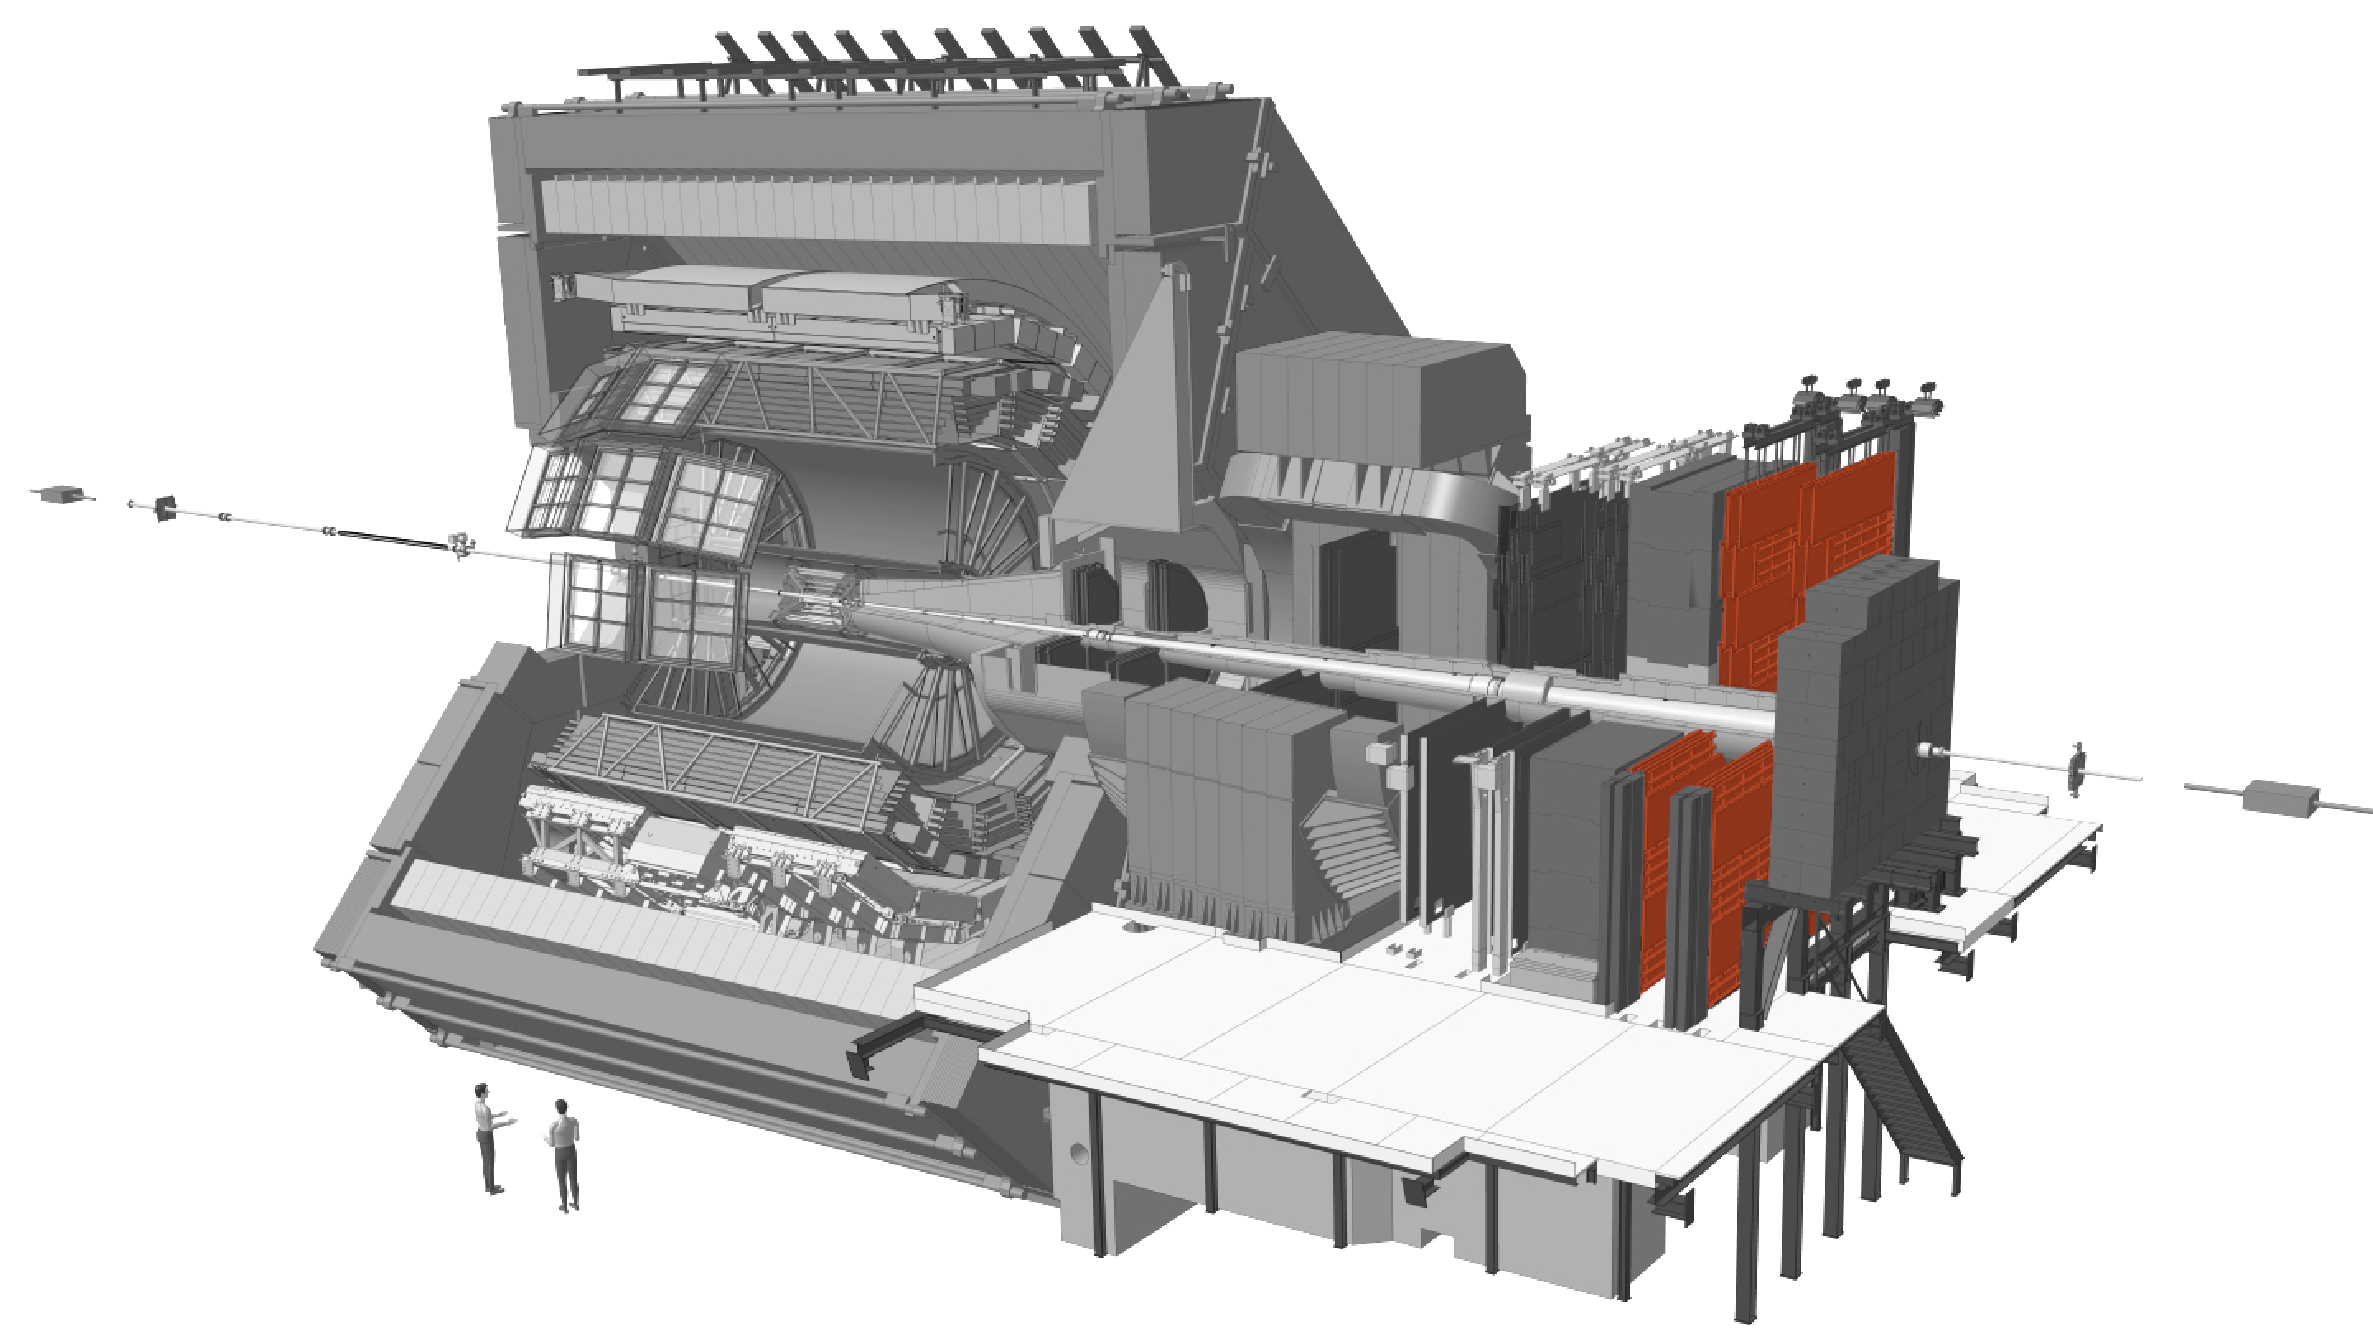
\includegraphics[width=\linewidth]{Chapters/Performance/Figs/ALICEmuon_MTR.pdf}
\caption{Grayed out ALICE with highlighted muon chambers and muon trigger chambers.}
\label{fig:ALICEmuon}
\end{center}
\end{figure}

\section{MTR monitoring data sources}
The ALICE experiment is equipped with a complex safety and hardware monitoring system called Detector Control System (DCS).
This system is the interface that allows to remotely control the detector, modifying the value of the high voltage, power supply and electronics statuses of the detectors.
In addition to the interface role, the DCS is connected to a database which records the readings of all the sensors related to devices handled by the DCS.
For what concerns the MTR, the DCS is able to record, for each chamber, the current, HV and LV voltage and thresholds used for the electronics, as well as global gas flow, humidity and composition values.
% each chamber current, voltage, gas flow , humidity and composition as well as other control parameters such as the external LV used to set the electronics threshold and the VME infrastructure working parameters.
The read-out values are stored in a DCS database which can be accessed using custom Siemens WinCC applications in order to produce plots and trends for several variables over time.
The data points are saved in the DCS database following two guidelines.
First of all the values are stored in the database whenever a given threshold on percent variation, with respect to previously stored value, is passed.
Additionally a slow clock ($5$ minutes) triggers the storage of the current read value, in order to keep track of smaller variations as well as of the stability of a given system.
The DCS values are accessible trhough a web interface called DARMA (formerly AMANDA) by executing database-like queries and downloading structured text file.

% \begin{figure}[!t]
% \begin{center}
% 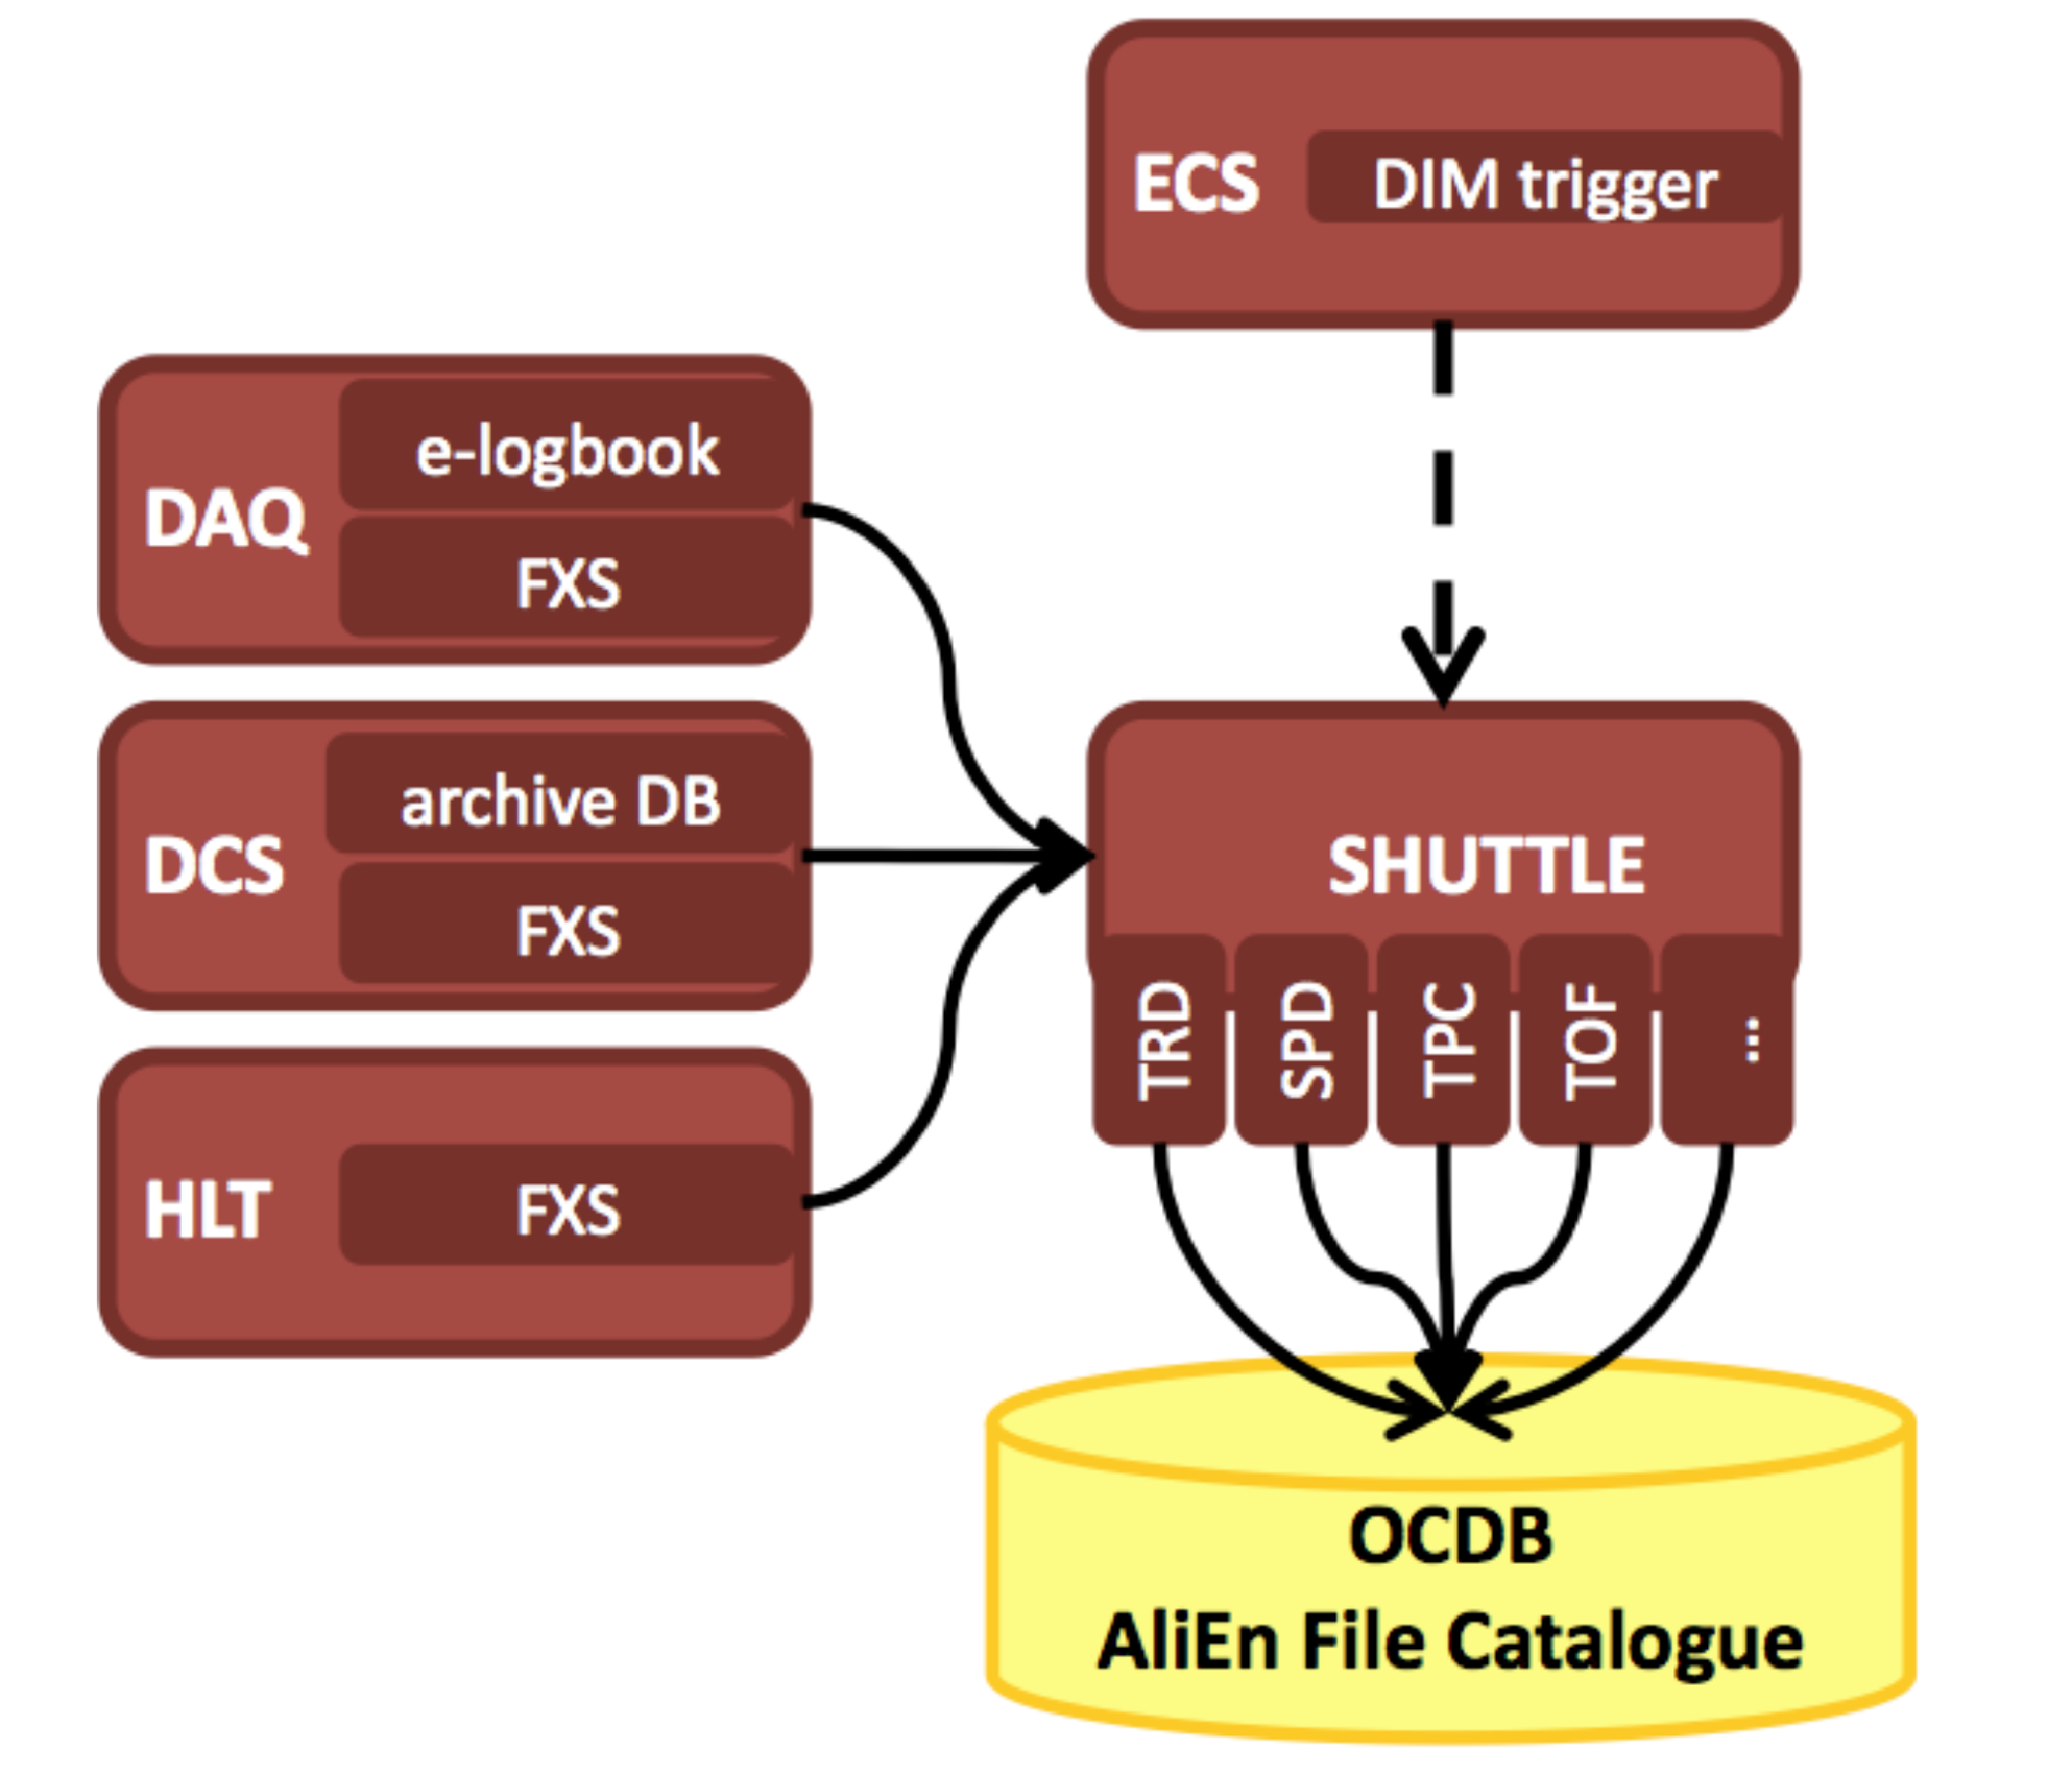
\includegraphics[width=0.7\linewidth]{Chapters/Performance/Figs/OCDB.pdf}
% \caption{Cartoon representing the data flow of collision data, DCS data and software infrastructure information. At the end of the run the Experiment Control System (ECS) sends the DIM trigger to the Shuttle, which is responsible of the migration of data in the GRID storage. The shuttle receives from the Data Acquisition System (DAQ), the Detector Control System (DCS) and the High Level Trigger (HLT) the information relative to the involved detectors. The data is packed together and moved to the GRID. From \cite{Zampolli:2010zz}.}
% \label{fig:shuttle}
% \end{center}
% \end{figure}

Some DCS information has to be available offline in order to perform offline reconstruction and simulation of the ALICE apparatus.
% The ALICE experiment status can be either data taking (when collecting physics data) or not.
A database, the Offline Conditions Data Base (OCDB), stores all the calibration and alignment data for such purposes.
A connection channel between the DCS infrastructure and the OCDB allows for the storage of the DCS readings during data taking.
This allows one to keep a track of the working conditions of the detectors, as well as of all of the information on the status of data taking, beam, etc. that are necessary to the reconstruction or to the realistic simulation of the detector.
% The OCDB is not a database in the usual sense.
All the data collected by ALICE is stored on the storage elements of the computing GRID.
% The files, in ROOT format, containing the stored data are not all stored in a single place.
% The OCDB provides a layer of access to those files, despite their geographical distribution.
In order to provide this access flexibility, the OCDB uses some parameters stored as file meta-data.
The data taking is organized in runs, periods of time of arbitrary length in which the detectors and accelerator conditions are considered to be stable.
The storage of information in the OCDB follows the same pattern.
% One of these meta-data is a validity interval defined using run numbers.
% It appears clear, at this point, that the OCDB structure strongly depends on the run numbers and that measurements performed outside of a data taking run cannot be stored in the OCDB.
The OCDB allows for the storage of DCS reading only during data taking runs, in which at least one of the ALICE's detectors are being read out.

\section{MTR integrated charge measurements}
\label{currents}
As already stated the ageing of RPCs is assumed to be proportional to the integrated charge liberated in the gas gap, mostly via the chemical action of compounds created in the avalanche or discharge process.
% The largest damage to the detector is caused by the chemical action of the ionized gas on the RPC inner surface.
% In particular the biggest part of the damages is not caused by the ionizing potential of the radiations and particles, but by the ionized gas particles inside the gas gap and their chemical action of the RPC surfaces.
The ALICE muon trigger RPCs  have been ageing-tested up to a total integrated charge of $50 mC/cm^2$. 
It is interesting to compare such a value with those reached after years of operation at the LHC.
The integrated charge is obtained by time-integration of the current flowing through the detector. 
To this respect, the gas gap of an RPC sees a current flow which has four components (Eq. \ref{eq:itot}):
\begin{itemize}
\item Ohmic component: it is due to the low conductivity of the gas gap and of the structure of the chamber. This part of the current depends linearly on the applied voltage;
\item Environmental irradiation: natural or activated radiation sources of ionising radiation, as well as cosmic rays detected by the RPC;
\item Noise-induced current: due to spontaneous discharges in the gas gap following electron extraction from the cathode surface;
\item Physics-induced current: caused by ionizing particles produced in physics collisions.
\end{itemize}

\begin{equation}
\label{eq:itot}
i_{tot}=i_{ohm}+i_{env}+i_{noise}+i_{phys}
\end{equation}

The ohmic, environmental and noise-induced components are always present, in case the detector is kept at the nominal working voltage.
The fourth component of the current depends on the operations of the LHC and the collision luminosity.
From an aging point of view the ohmic current is not expected to have an effect on the detector ageing, as it is not associated to the liberation of charges in the gas, then it should not be taken into account in the computation.
The environmental current is always present and can cause aging effects, but its entity is negligible.
The noise-induced current is relevant for aging effects.
% For this reason, it is difficult to measure the noise-induced current.

A detector might be switched on and fully operational when no data taking is being performed, for example, between one run and the following one or when no beam is provided by LHC and ALICE is taking cosmic data.
In this kind of situations the amount of current flowing trough the system corresponds to the sum of the ohmic contribution and the environmental and noise-induced ones.
Measuring the amount of current flowing in a chamber in these conditions would provide a measurement of the dark current $i_{dark}$, defined as:

\begin{equation}
\label{eq:idark1}
i_{dark}=i_{env}+i_{ohm}+i_{noise}
\end{equation}

Given that $i_{env}$ is negligible, it can be removed, obtaining a measure of the dark current:

\begin{equation}
\label{eq:idark}
i_{dark}\approx i_{ohm}+i_{noise}\ \ \ for\ \ \ i_{env}\rightarrow0
\end{equation}

Ideally, to obtain a precise evaluation of the current causing aging of an RPC, one should integrate:

\begin{equation}
\label{eq:inet}
i_{net}=i_{env}+i_{phys}+i_{noise}
\end{equation}

Since it is not possible to extract $i_{ohm}$ from $i_{dark}$ two extreme approaches are possible, assuming the $i_{dark}$ value can be dominated by either of its terms.
If $i_{dark}=i_{ohm}$ the dark current contribution to $i_{tot}$ must be subtracted to obtain the value of $i_{net}$ which causes aging effects, hence $i_{net}=i_{tot}-i_{dark}$.
If $i_{dark}=i_{noise}$, its contribution to $i_{tot}$ may take part in aging effects, hence $i_{net}=i_{tot}$.

In either cases, the integration of $i_{net}$ over time will provide the aging index that can be compared to the limit value obtained in the tests.
The newly introduced framework allows for both approaches.
All the integrated charge shown in this thesis have been obtained assuming $i_{dark}\approx i_{ohm}$.
% A doubling of the integrated charge value has been observed using the assumption of $i_{dark}\approx i_{noise}$ instead, even if the plot shape is qualitatively the same.

The above-mentioned measurements are not possible using OCDB as the only data source.
In fact the OCDB polls DCS readings and stores them permanently only when data taking is being performed.
Even if this condition can happen both with beam collisions and during cosmic runs, the coverage of the dark periods of the MTR is partial.

The work presented in this chapter was originated from the idea of combining OCDB and DCS measurements using the well established OCDB data retrieving interface and the AMANDA/DARMA DCS database access tool, in order to increase the working conditions coverage with respect of the OCDB-only approach.
In addition the granularity provided by the DCS is much better with respect to the one of the data propagated to the OCDB, but the DCS readings have no run number, beam condition or LHC status information.
By combining the two data sources a better understanding of the MTR performances would arise, giving the possibility to perform trend and distribution studies, as well as correlation studies between MTR parameters and external conditions such as collisions luminosity.

\section{MTR performance analysis framework}
As a subject of this thesis a brand new analysis framework for MTR performance analysis has been developed.
This framework main task is to combine the data coming from OCDB and AMANDA/DARMA in order to create a complete set of data which can be used for specific studies of trends and correlations concerning the MTR system.
As an additional value to this project, the framework aims at providing a reliable tool which is accessible and open source.
Having a centralized repository, with the possibility of participating to the development of the framework and to the fixing of eventual software bugs, can improve both the user experience and the number of users hence the bug detection capability.

The framework internal data format is filled on a per-run basis, and contains the following information:
\begin{itemize}
\item Run number: identifies the current run;
\item Start and End of Run (SOR and EOR): Are the timestamps defining the data taking inside a run;
\item Average HV: average value (weighted over time) of supplied HV. One value per each of the 72 RPCs;
\item Average $i_{tot}$: average value (weighted over time) of supplied current.  One value per each of the 72 RPCs;
\item Average $i_{dark}$: average value (weighted over time) of dark current, extrapolated via the algorithm.  One value per each of the 72 RPCs;
\item Integrated charge: integral of the $i_{net}$ over the run.  One value per each of the 72 RPCs;
\item Bending scalers: total number of hits on the bending plane of the chamber.  One value per each of the 72 RPCs;
\item Non-bending scalers: total number of hits on the bending plane of the chamber.  One value per each of the 72 RPCs;
\end{itemize}

% The framework is composed by two acting classes.
% The first, \code{MTRShuttle}, is the one which performs the data retrieving, parsing and manipulation.
% It is responsible of merging the data coming from the two sources and of creating a vector of \code{RunObject}s to store the data.
% The second class is \code{MTRBooster} which elaborates the \code{RunObject}s vector created by \code{MTRShuttle} and presents to the user the possibility to generate trend and correlation plots using a friendly interface for the specification of the plot options.

% The \code{RunObject} arrays are filled by a \code{MTRShuttle} instance using data coming from OCDB and DCS database.
% Their filling is performed using a either a local or a remote copy of the OCDB and a local copy of the DCS database.
% Several steps are performed by the filling algorithm.
The algorithmic steps performed to obtain the $i_{net}$ values over time are:
\begin{enumerate}
\item DCS $i_{tot}$ and $HV$ data points are retrieved;
\item OCDB data regarding beam conditions, HV readings and scalers values are stored;
% \item Additional dummy runs are created, filling the periods between runs whose information is found on the OCDB;
\item Current readings are flagged as "dark" using the OCDB information about beam presence. See schema in figure \ref{fig:iDarkFlag};
\item A linear interpolation of all the $i_{dark}$ values is performed. 
% Each current reading has two floating point values corresponding to $i_{tot}$ and $i_{dark}$. For values flagged as dark the two values are equal. 
For all the non-dark current readings the value of $i_{dark}$ is set using the interpolation of dark current values. See schema in figure \ref{fig:interpolation};
% \item For each \code{RunObject} the average $i_{tot}$ and $i_{dark}$ values are computed via the weighted average of all the $i_{tot}$ and $i_{dark}$ falling between the SOR and the EOR;
% \item For each run the integral over time of the $i_{net}$ values is performed and stored in the relative \code{RunObject}.
\end{enumerate}

\begin{figure}[!t]
\begin{center}
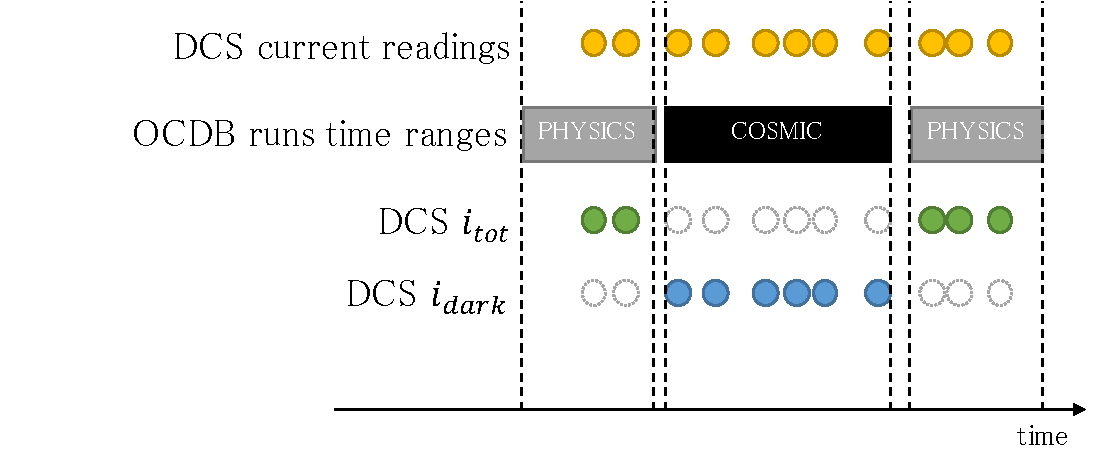
\includegraphics[width=0.8\linewidth]{Chapters/Performance/Figs/darkCurrentFlagging.pdf}
\caption{Cartoon representing the process of dark current readings flagging by combining OCDB and DCS data. The lines are represented on an arbitrary horizontal time axis. 
The first line represents the current readings stored in the DCS database. 
The frequency of those measurements is not fixed. 
The second line represents with boxes the duration of several runs. 
Gray boxes show physics runs, while the black box represents a run in nominal conditions without beam (cosmic run). 
The first line currents can be flagged either as $i_{tot}$ if within a non-cosmic run or as $i_{dark}$ otherwise. 
They are represented in the last two lines accordingly. }
\label{fig:iDarkFlag}
\end{center}
\end{figure}

\begin{figure}[!t]
\begin{center}
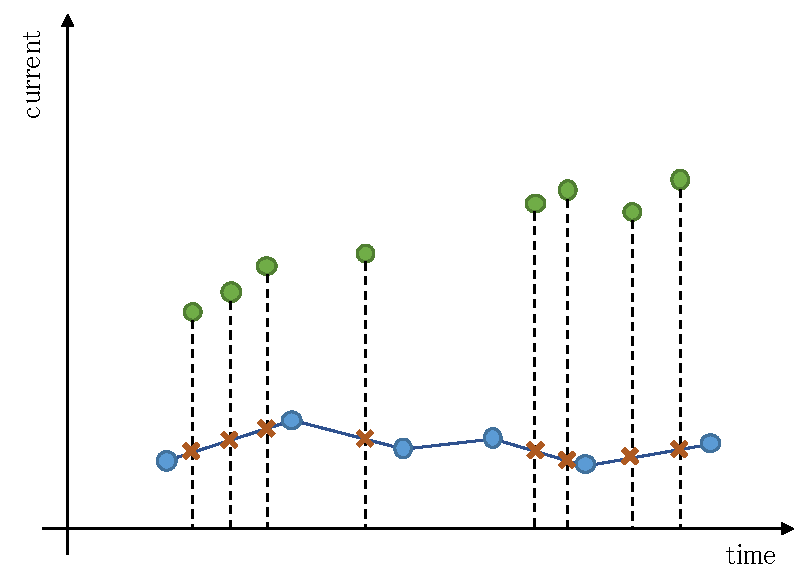
\includegraphics[width=0.8\linewidth]{Chapters/Performance/Figs/interpolation.pdf}
\caption{Cartoon representing the interpolation process.
The green and blue points represent $i_{tot}$ and $i_{dark}$ readings, according to figure \ref{fig:iDarkFlag}.
The dashed vertical lines represent the projection on the time-axis of $i_{tot}$ readings.
The solid line connecting $i_{dark}$ measurements represents the linear interpolation.
The crossings between the $i_{dark}$ interpolation curve and the vertical dashed lines, are the $i_{dark}$ values attributed to $i_{tot}$ measurements.
Such values are highlighted with red crosses.}
\label{fig:interpolation}
\end{center}
\end{figure}

% Once the data parsing has been accomplished the plots can be created via an instance of \code{MTRBooster}.
% Several methods are presented to the user in order to specify the plot one wants to create.
% These methods are described in details here after:
% \begin{itemize}
% \item \code{SetPlane},\code{SetSide} and \code{SetRPC}: optional methods to request a plot specific for a given RPC. The default value causes all the RPCs to be plotted in different colors. For example calling \code{SetPlane} and not the other two methods causes the plot to show all the RPCs belonging to the selected MTR plane. Same goes for calling only \code{SetSide};
% \item \code{SetX} and \code{SetY} are the mandatory methods which allow the user to select what \code{RunObject} data to use as $x$ and $y$ coordinate in the plot. Selecting one of the available timestamps as $x$ value produces a trend plotRange setters: methods to set the time frame in which the data have to be plotted are provided. A set of three methods (\code{SetRange(min,max)},\code{SetMin(min)} and \code{SetMax(max)} is provided for setting the range using timestamps, run numbers or human readable dates;
% \item Run selections: methods to select standard types of runs are provided. One can easily plot only runs with nominal HV value, runs with beam presence, runs without beam, runs with nominal HV and no beam and runs adequate for the integrated charge computation;
% \item \code{AccumulateY}: this method makes the plotter integrate the $y$ values while plotting. Since each run has the value of integrated charge within the run, this option is needed to provide the amount of integrated charge over the whole analyzed period;
% \item \code{NormalizeToArea}: the $y$ values (and the $x$ ones if not a trend plot) are divided by the RPC area to provide a value over $cm^2$;
% \item \code{PlotAverage}: superimposes to the generated plot the average behavior of the plotted RPCs;
% \item \code{PlotMinMax}: superimposes to the generated plot the two plots of the RPCs whose last point is the highest and lowest of the plotted set of RPCs.
% \end{itemize}

The framework has been extensively tested and the plots presented in the following sections of this thesis have been produced by means of the new framework, merging the two available data sources for the first time.

% \section{Data selection}
% The objective of this analysis was to perform a performance study of the ALICE muon trigger's RPCs throughout the whole operative life of the detectors, namely from 2010 to current days.
% % While the retrieval of DCS data for the whole period is trivial since the only possible selection is timestamp-based, the data downloaded from the OCDB can be selected using several flags.

% In order to opportunely flag the DCS current readings either as dark or not it was needed to select runs with no beam and nominal HV supply.
% After some tests the choice converged on the selection of special runs for cosmic ray data taking, for which there is no collision in the LHC and the muon trigger RPCs are set to the nominal working voltage.
% % In fact these runs are the only ones which guarantee the data taking was performed without collisions or beam presence and that the muon trigger was set at the nominal working HV.
% Another run-kind candidate was the CALIBRATION type, which characterizes runs which are performed normally at the end of a data taking run in order to check the status of the front-end electronics.
% The CALIBRATION run refers to two kind of diagnostic run lasting for 2 minutes each.
% The first is a software-triggered read-out of the whole detector performed without collisions in the LHC, aimed at spotting noisy channels.
% During the second CALIBRATION run type the whole FEE is artificially stimulated and read-out in order to detect dead channels.
% % Even if normally these runs are performed with the detector at nominal HV they are often repeated with the detector moved in safe position (i.e. around $8500V$) and/or some beam movements and modifications in the LHC.
% The detector is usually at nominal working voltage during these runs. 
% However, they can occasionally be performed with a reduced HV and/or during the presence of beam modifications in the LHC.
% % The comparison of the new framework with and independent algorithm tested as right provided some checks: the selection of CALIBRATION runs was leading to a wrong estimation of the dark current, while using the COSMIC runs the two algorithms converged at the same results.
% A total of around $5200$ cosmic runs have been used for this analysis.

% The scalers values are not stored in the DCS database, hence it is necessary to download OCDB information for all the runs performed with beam presence and collisions in the LHC.
% More than $12000$ runs have been selected, covering $pp$, $p-Pb$ and $Pb-p$, $Pb-Pb$ and $Xe-Xe$ colliding systems at all the center of mass energies provided by the LHC since the beginning of the operations.

\section{Determination of dark current and dark rate and dark current interpolation procedure}
One crucial point is how to determine if a rate or a current reading are indeed "dark" readings.
While the dark current definition has already been quoted in section \ref{currents} the dark rate definition will be given.

% The dark current is the measurement of current which physiologically flows trough the detector when it is supplied with working point HV and no collision-induced irradiation is present (e.g. when no beam is present in the LHC).
% This current has an ohmic component and an irradiation one, the second caused by environmental radioactivity and cosmic rays reaching the detector.
The dark rate is the rate observed and measured in the same conditions as the dark current, i.e. at nominal HV and when no collision is taking place in the LHC.
This rate should be correlated with the natural radioactivity and cosmic rays incidence, as well as intrinsic noise counts of the detectors, but may contain a contribution related to noisy read-out channels.
% In addition, since the dark rate is read-out by the electronics, dead channels might cause blind spot which in turn makes the rate to be lower than expected.

The dark runs can be defined in various ways.
In order to properly flag the DCS current readings either as dark or not it was needed to select runs with no beam and nominal HV supply.

Selecting runs taken with physics setup without beam presence (flagged as "COSMIC") are the safest choice, but this kind of runs is less frequent and provides less coverage of the operation period.

Selecting calibration runs allows to better cover the operation period, since at least two calibration runs are performed at the end of every physics fill of the LHC.
The CALIBRATION run refers to two kind of diagnostic run lasting for 2 minutes each.
The first is a software-triggered read-out of the whole detector performed without collisions in the LHC, aimed at spotting noisy channels.
During the second CALIBRATION run type the whole FEE is artificially stimulated and read-out in order to detect dead channels.
Within a CALIBRATION run the detector is usually at nominal working voltage.
However, they can occasionally be performed with a reduced HV and/or during the presence of beam in the LHC.

% Measurements of dark current trends using cosmic or calibration runs only are displayed in figures \ref{fig:iDarkCOSMIC} and \ref{fig:iDarkCALIB}.
% Assuming that the dark current should be constant without beam presence, one can observe a strange behavior for dark current computed using calibration runs only.
% In particular the dark current trend following a period with beam presence shows a non negligible slope which causes an overestimation of the $i_{dark}$.
% % Some dark current variations which aren't completely understood are present.
The dark current trend using cosmic runs only is displayed in figure \ref{fig:iDarkCOSMIC}. 
As for calibration runs, it was observed that the dark current measured immediately after a physics fill (which is when most calibration runs are performed) is systematically higher that that measured in “quiet” periods. 
The understanding of this effect is the fact that after a period of operation with beam presence some impurities stay in the gas gap for a while before being fluxed by the gas system.
% Such impurities affect the chamber conductivity locally, provoking discharges that in turn induce a temporary raise of the dark current.
In order to avoid instabilities in the interpolation procedure due to this effect, this work uses only cosmic runs to estimate the dark current and dark rate values.

\begin{figure}[!t]
\begin{center}
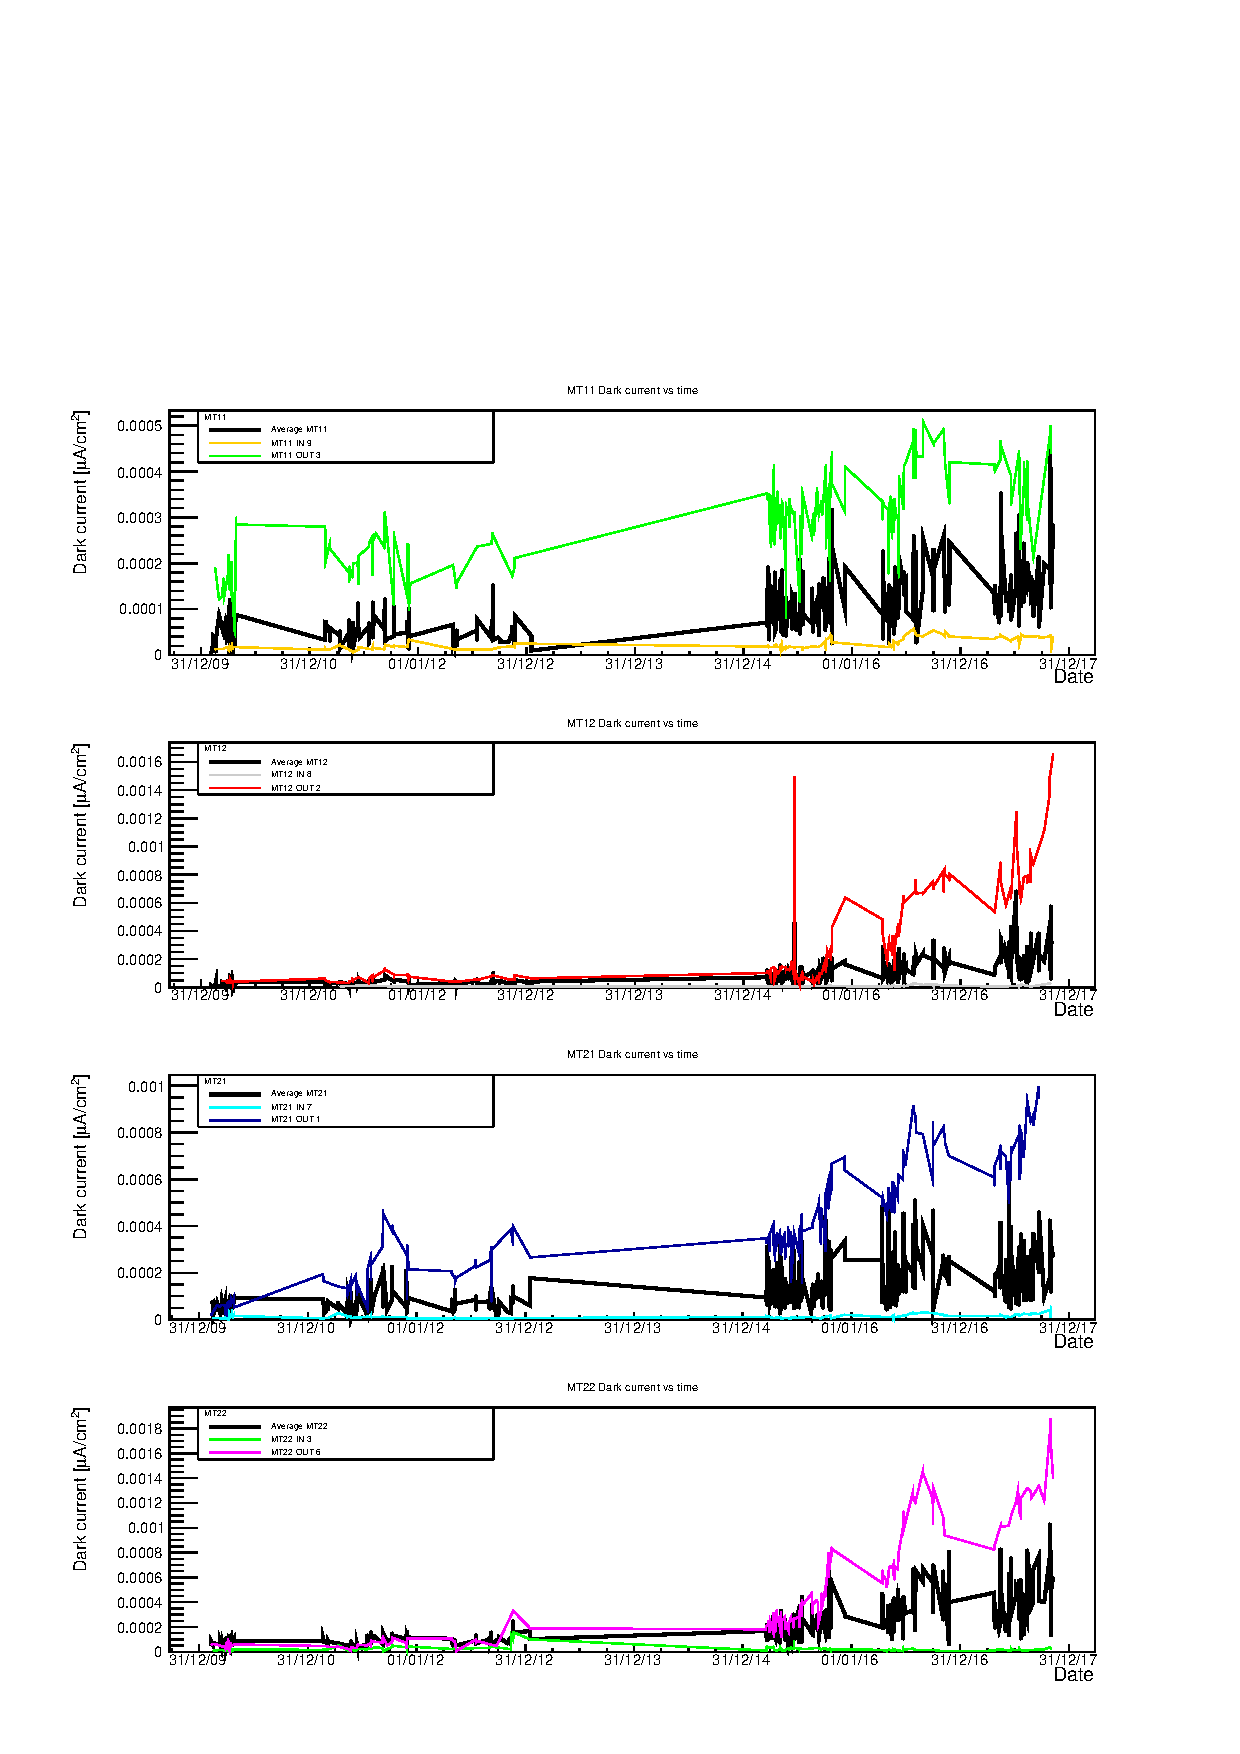
\includegraphics[width=0.95\linewidth]{Chapters/Performance/Figs/iDark_COSMIC_minmax.pdf}
\caption{Average dark current trend computed with the described procedure using cosmic runs only. The trends are divided by plane (from top to bottom MT11, MT12, MT21, MT22). For improved readability for each plane only the maximum and minimum trends and the average plot are shown. Each point corresponds to a run. The $y$ value is obtained via the average of all the RPCs dark currents, while the $x$ value is the timestamp which corresponds to the end of run.}
\label{fig:iDarkCOSMIC}
\end{center}
\end{figure}

% \begin{figure}[!t]
% \begin{center}
% 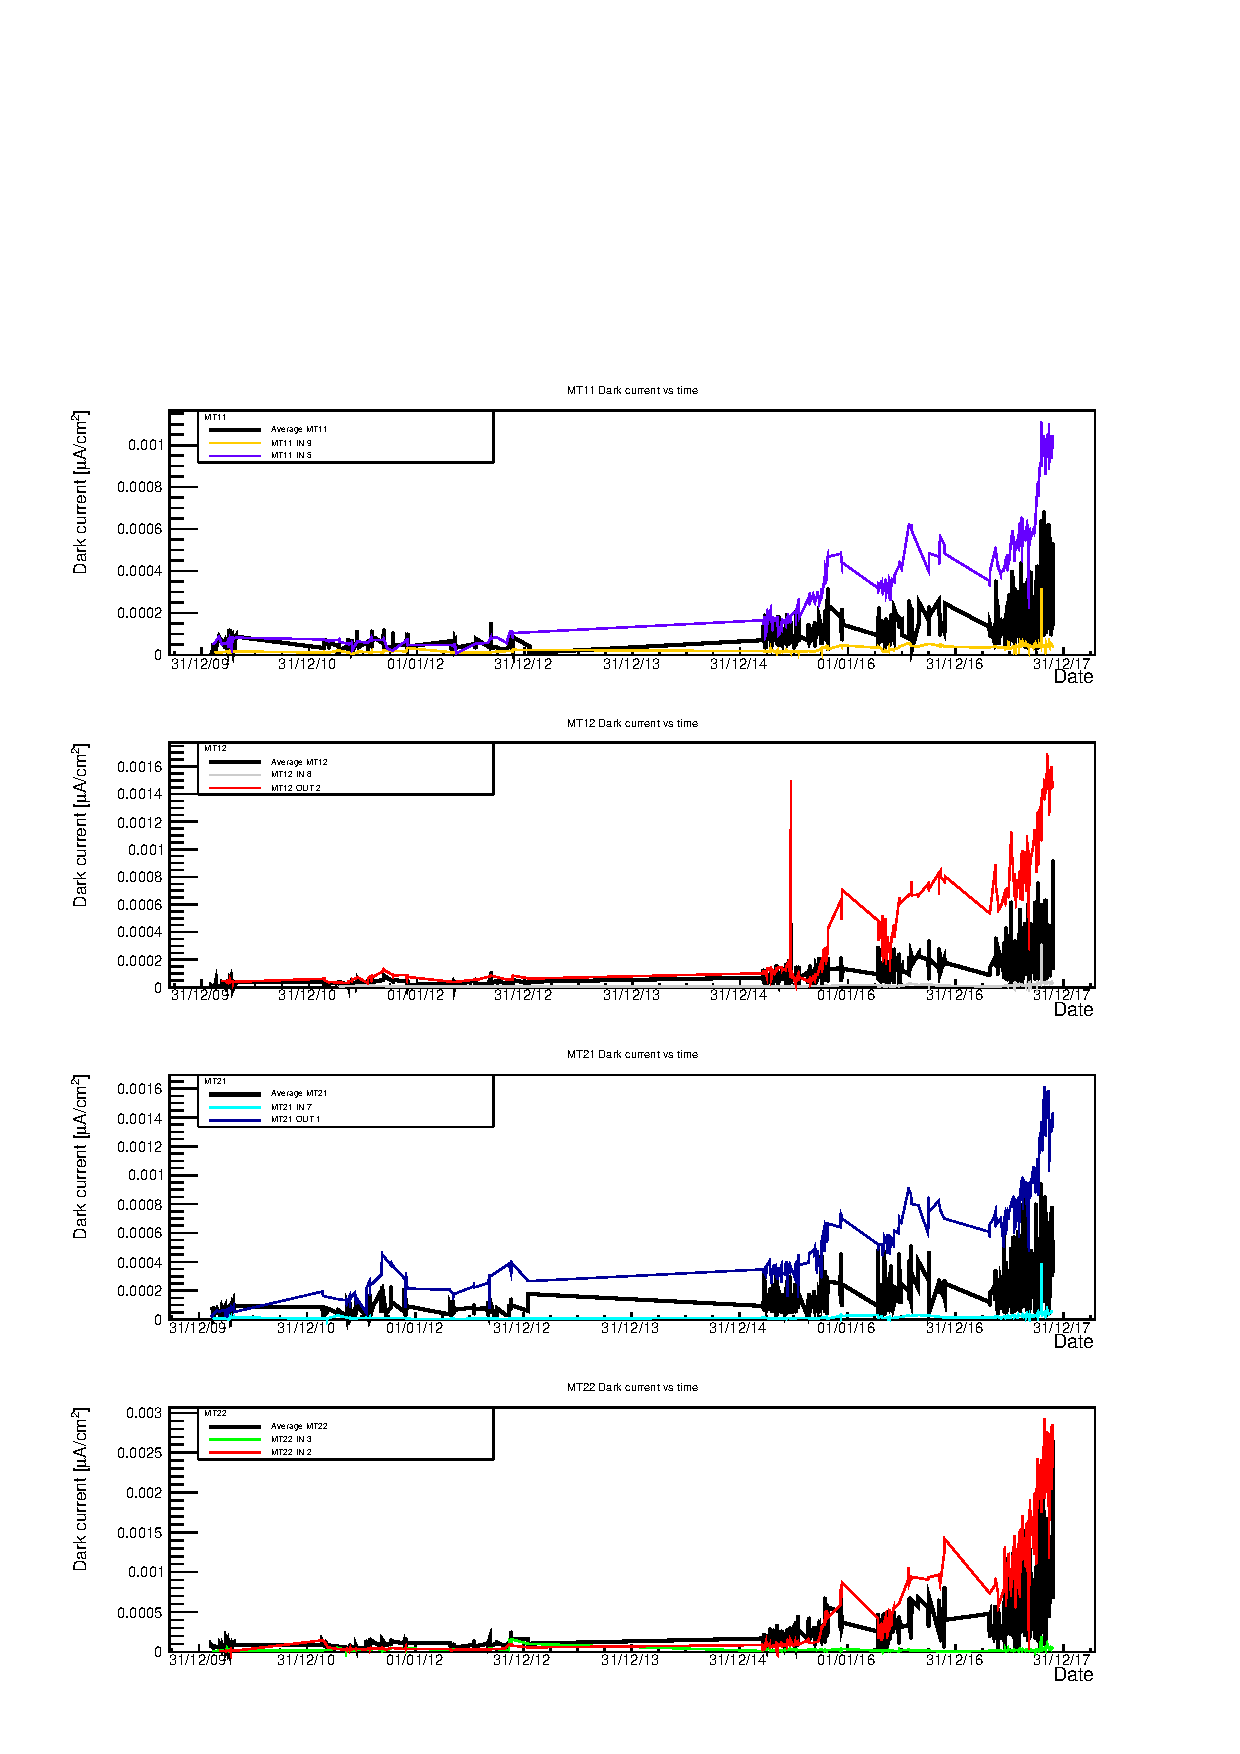
\includegraphics[width=0.95\linewidth]{Chapters/Performance/Figs/iDark_CALIB_minmax.pdf}
% \caption{Average dark current trend computed with the described procedure using calibration runs only. The trends are divided by plane (from top to bottom MT11, MT12, MT21, MT22). For improved readability for each plane only the maximum and minimum trends and the average plot are shown. Each point corresponds to a run. The $y$ value is obtained via the average of all the RPCs dark currents, while the $x$ value is the timestamp which corresponds to the end of run.}
% \label{fig:iDarkCALIB}
% \end{center}
% \end{figure}

A total of around $5200$ cosmic runs have been used for this analysis.
The scalers values are not stored in the DCS database, hence for the rate computation it is necessary to download OCDB information for all the runs performed with beam presence and collisions in the LHC.
More than $12000$ runs have been selected, covering $pp$, $p-Pb$, $Pb-Pb$ and $Xe-Xe$ colliding systems at all the center of mass energies provided by the LHC since the beginning of the operations.

% At the moment of deciding which procedure to adopt to perform the dark current interpolation, in order to assign dark current values to non-dark current readings, two possibilities were spotted:
% \begin{enumerate}
% \item The interpolation is a moving linear fit performed on a group of $N$ dark current readings;
% \item The interpolation is the line connecting the two immediately surrounding dark current readings.
% \end{enumerate}

% While the first option is less sensible to overestimation caused by localized spikes, extending the set of currents to a fixed number $N$ of readings might make the algorithm take in account readings which are far in time with respect to the measurements for which the dark current value has to be set.
% By doing so the risk of taking dark current readings extending over a time range in which non-recorded modifications of the detector state happened is high.
% If, for example, the detector has been switched off for a while and switched on between the set of $N$ readings, some dark current readings will correctly represent the latest detector status, while the ones preceding the switch off will induce an overestimation of the dark current on the algorithm.
% For these reasons, in order to limit the injection of artifacts by the algorithm, the second approach has been selected.
% For the sake of completeness one should point out that the second option is equivalent to the first one in which $N=2$.
% From an operative point of view this grant the additional advantage of avoiding a time consuming set of linear fits, replacing the minimization procedure with the analytic solution for a line segment crossing two points.

\section{Performance analysis}
Several aging indicators for the 72 RPCs of the ALICE muon trigger will be presented and commented, trying to highlight eventual problematic RPCs which should be replaced.
A particular focus on the FEERIC-equipped RPC will address the main differences between the old and new read-out electronics from the chambers operations point of view.
% In order to improve the performances and the rate capability of the current detectors a new amplified electronic read-out board has been developed.

% The current read-out board is called ADULT and was developed to allow for a switch between streamer and avalanche operation modes through a dual threshold discriminator with modifiable thresholds.
% Even if ADULT performed well, the streamer mode was never used in the muon trigger RPCs.
% The signal dynamics of an avalanche is much smaller than that of a streamer, since only in the latter in gas multiplication is possible.

% Based on these two arguments, a new single threshold electronically amplified electronic read-out board has been developed.
% This new board is called FEERIC and is specialized in reading signals coming from avalanche operation mode and adopts a mosfet amplification stage.
% The effects of an amplified electronics are various.
% First of all the required charge dynamics in the gas gap is much lower with respect to that required by an non-amplified read-out.
% The free charge of the signal is in fact collected by the electrodes and amplified out of the gap.
% Lowering of the charge per hit allows to have smaller dead times since restoring the original HV requires less energy.
% Requiring a lower charge has the side effect of allowing a reduction of the operating HV, which leads to a even faster recovery time.
% The drawback of the adoption of an amplified electronics is that small noise signals, which a non-amplified electronics does not detect, might become observable and detected.

% One RPC currently part of the ALICE muon trigger is equipped with the new read-out electronics since 2015.
% In all the following plots the first part of the RPC operations is shown for the sake of comparison, despite the fact that it has been equipped with the FEERIC front end only from that date.
% % While this test sample wasn't the finalized electronics, which will be instead installed on all the RPCs by the beginning of RUN3, an insight of the improved performances is already possible.
% The RPC equipped with the FEERIC read-out offered an insight of the improved performances.

% After several tests the HV for the FEERIC equipped RPC has been set to $9800V$ gaining around $500V$ with respect to ADULT-equipped RPCs without modifying the detection efficiency of the detector.

\subsection{Dark current trend}
The evaluation of the dark current trend is fundamental to understand the health of the inner surfaces of the detectors.
This working parameter strongly depends on the presence of irregularities on the boundary surfaces of the RPCs, hence can be used as a diagnosis tool.
% In figure \ref{fig:iDark4Planes} a view of the trends of the dark current measurements as a function of time (date) is presented, each panel corresponds to the trends of the RPCs installed in MT11, MT12, MT22 and MT21 from top to bottom.
The dark currents as a function of time for the 4 different RPC layers is shown in the four panels of figure \ref{fig:iDarkCOSMIC}. 
In each panel, the average dark current of the layer as well as the trend for the RPC drawing the largest and the smaller current in that layer are shown.
The dark current measurements are reported in $\mu A/cm^2$, since dark current values have been divided by the corresponding RPC area.
Given that the RPC areas are not all the same, this procedure helps to produce results which can be compared.

% \begin{figure}[!t]
% \begin{center}
% 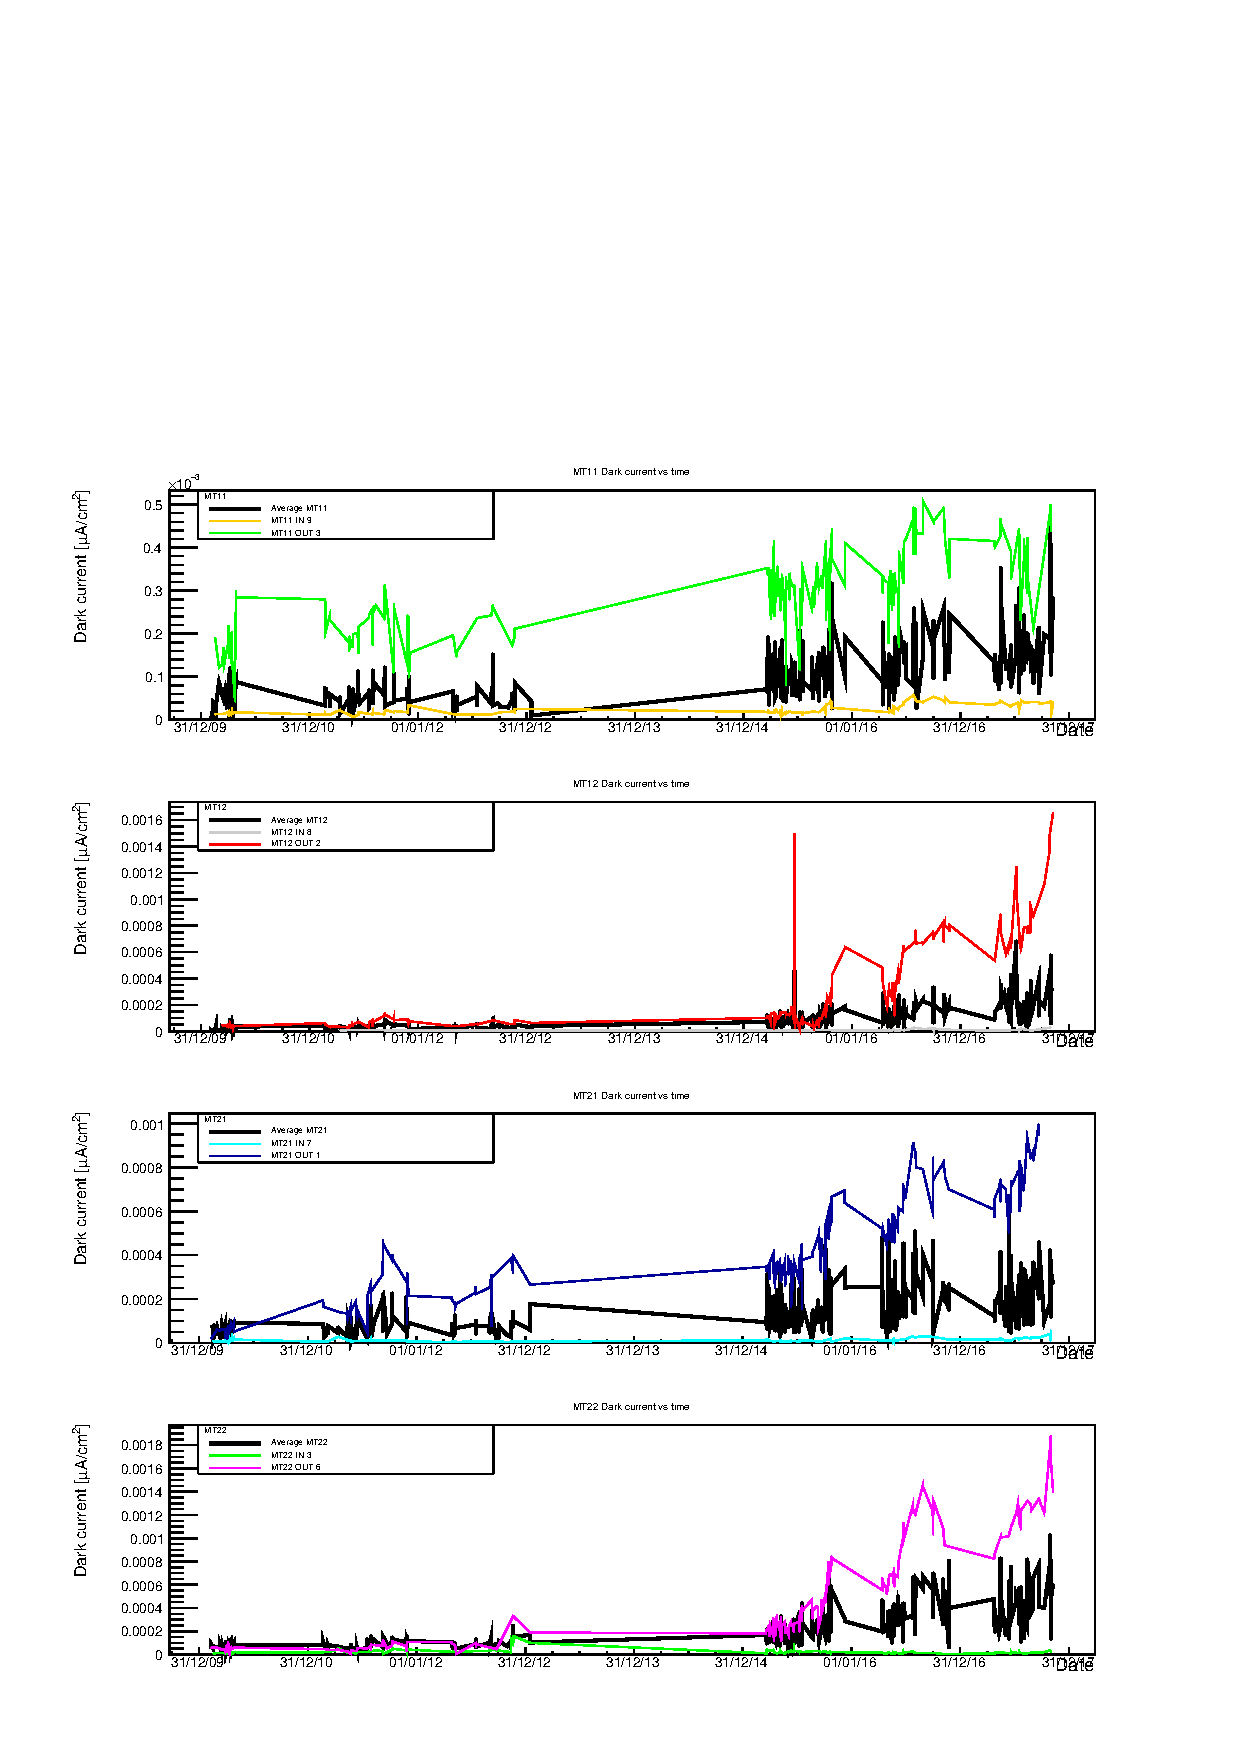
\includegraphics[width=0.95\linewidth]{Chapters/Performance/Figs/iDark4PlanesMM.pdf}
% \caption{Dark current trends for each RPC over the whole operation period. The trends are divided by plane (from top to bottom MT11, MT12, MT21, MT22). For improved readability for each plane only the maximum and minimum trends and the average plot are shown. Each point corresponds to a run. The $y$ value is obtained via the average over time of the dark current measurements, while the $x$ value is the timestamp which corresponds to the end of run.}
% \label{fig:iDark4Planes}
% \end{center}
% \end{figure}

Sometimes a reduction of the dark current value can be observed.
This effect is more important and clearly noticeable at the beginning of each year.
It is commonly accepted that such a reduction of the dark current is caused by the yearly winter shutdown which undergoes for all the CERN LHC facilities.
In fact every year the beam operations are stopped for a winter period which typically lasts from late November to the first 3-4 months of the following year.
During this period the irradiation caused by the beam operations is absent.
At the same time the gas flow trough the chambers extracts impurities and eventually improves the inner surfaces smoothness.
This recovery effect causes a reduction of the dark current and can systematically be observed for all the RPCs.

The trend shown in figure \ref{fig:iDarkCOSMIC} covers four years of operations and includes the first LHC long shutdown period (LS1).
A different trend before LS1 has been observed with respect to the one measured during RUN2.
The dark current seems to raise during the RUN2 operations.
The reason of such behaviour might be related to the much higher luminosity observed in RUN2, hence the stronger irradiation of the chambers causing longer recovery times.
Comparing the specific trends of each RPC with the average trend one can easily observe that the increase of the average trend is mostly caused by some outliers.
In fact around 4/5 RPCs per plane, over a total of 18, show a dark current value large than the average trend.
This behavior indicates that most of the RPCs present a much more stable behavior.
The outliers of this trend can be considered the worst case scenario and should be monitored with attention in order to promptly notice eventual worsening of performances.

A detailed view of the dark current measurements for the FEERIC-equipped RPC are reported in figure \ref{fig:FEERICiDark}.
The dark current of the FEERIC RPC is negligible and in average a factor $20$ lower with respect to the average.
It is important to notice that while all the other RPCs show an increase of the dark current over the years of operation, the measurements of dark current performed on the RPC equipped with the amplified electronics are compatible with a constant behavior.

\begin{figure}[!t]
\begin{center}
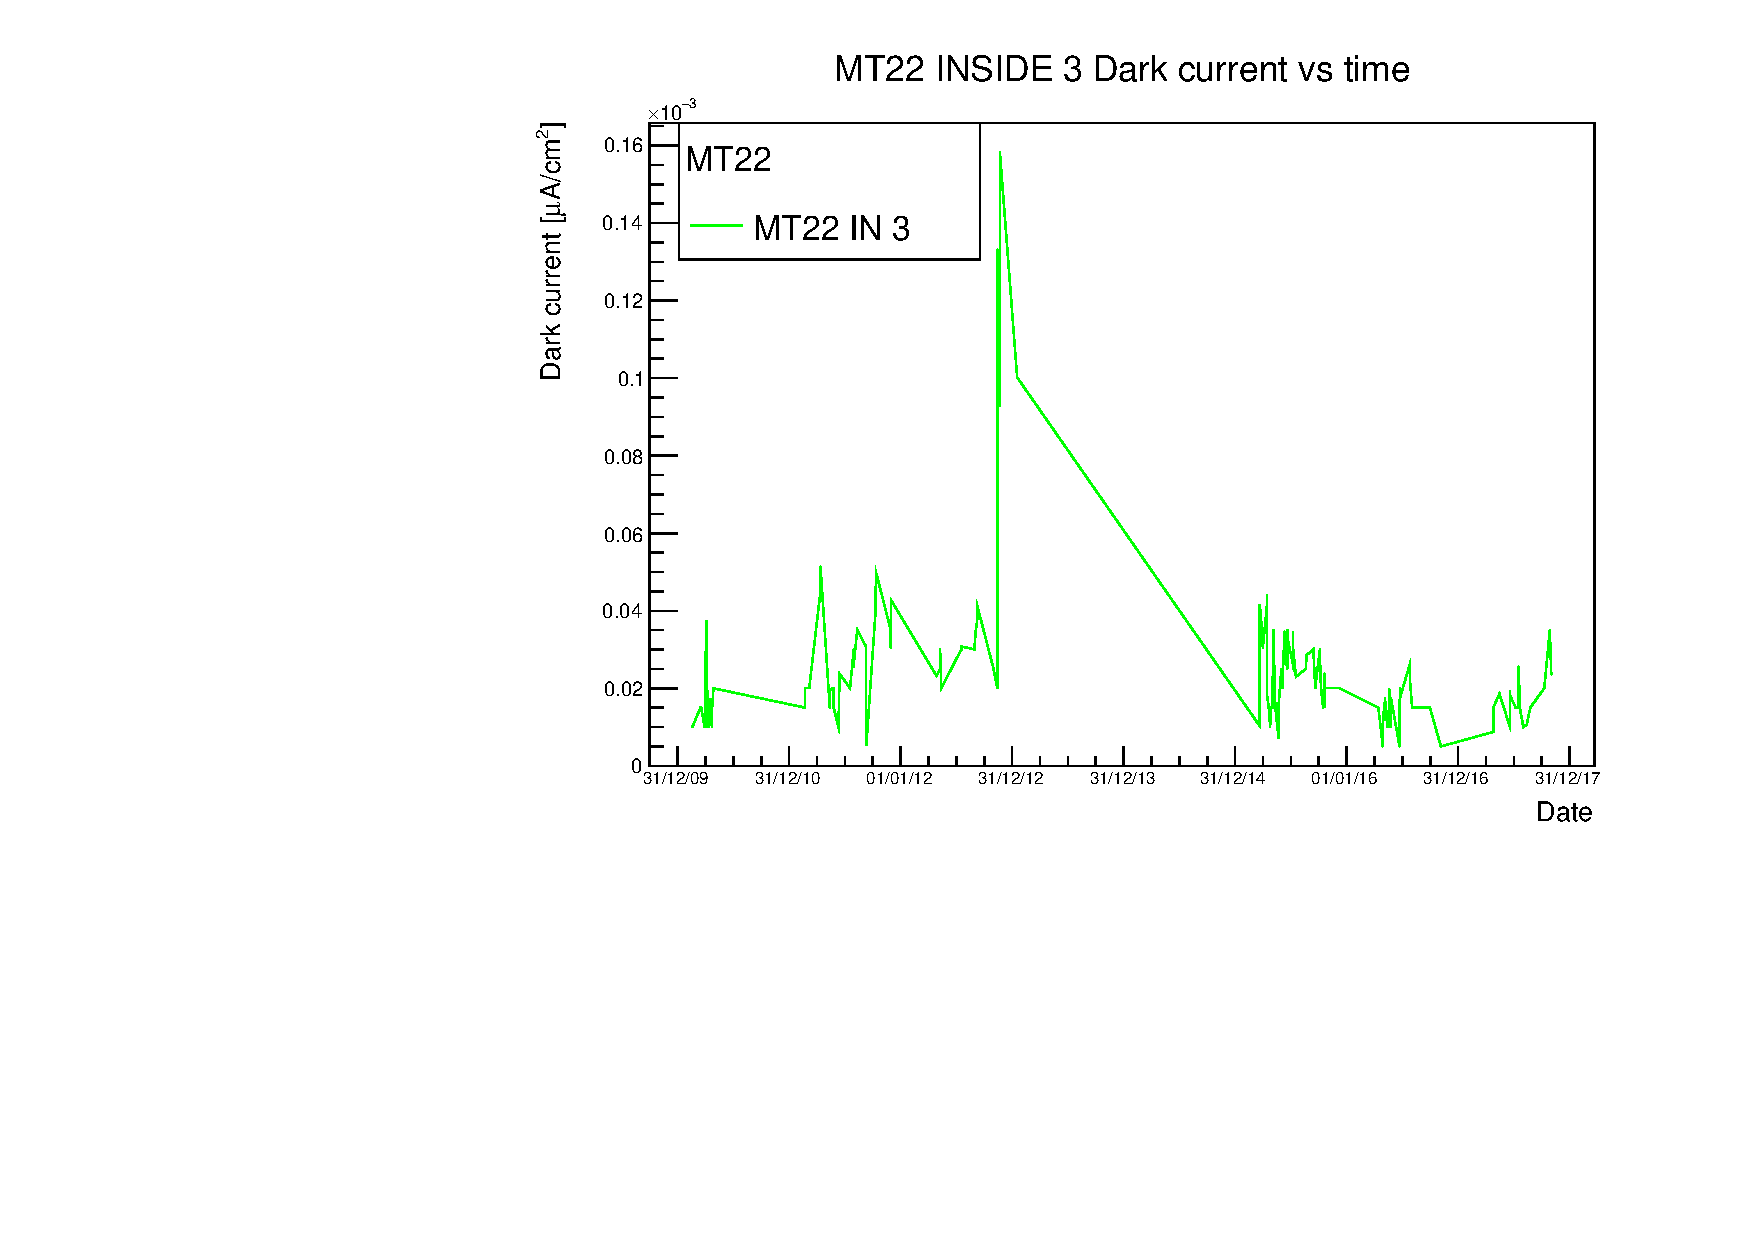
\includegraphics[width=0.95\linewidth]{Chapters/Performance/Figs/iDarkFEERIC.pdf}
\caption{Dark current as a function of time for the FEERIC-equipped RPC. The FEERIC FEE has been installed in 2015, hence the first part of the plot refers to the same RPC equipped with the ADULT front-end. The dark current is measured during cosmic runs.}
\label{fig:FEERICiDark}
\end{center}
\end{figure}

\subsection{Net current and integrated charge trend}
This work presents for the first time a method to combine data from OCDB and DCS databases capable of subtracting the contribution of dark current from the evaluation of the integrated charge.
In order to do so the net current should be evaluated starting from the total current and the dark current readings, through the procedure presented in the previous sections.

The net current measurements are reported in figure \ref{fig:iNet4Planes} as a function of time (date).
The panels correspond to the trends of MT11, MT12, MT21 and MT22 from top to bottom.
In each panel, the average net current of the layer as well as the trend for the RPC drawing the largest and the smaller current in that layer are shown.
The net current measurement represents the current related merely to the irradiation of the detectors, hence it is expected to have a baseline at $0\ \mu A/cm^2$ and increases with the intensity of the beam.
The expected behavior is observed through the whole time range.

\begin{figure}[!t]
\begin{center}
\includegraphics[width=0.95\linewidth]{Chapters/Performance/Figs/iNet4PlanesMM.pdf}
\caption{Net current trends for each RPC over the whole operation period. The trends are divided by plane (from top to bottom MT11, MT12, MT21, MT22). For each plane only the trends of the RPC with the maximum and minimum current are shown. Each point corresponds to a run. The $y$ value is the difference between the average total and dark currents, while the $x$ value is the timestamp which corresponds to the end of run.}
\label{fig:iNet4Planes}
\end{center}
\end{figure}

% Concerning the FEERIC-equipped RPC, the net current measurements shown in figure \ref{fig:FEERICiNet} present a similar improvement effect already observed for the dark current measurements.
Concerning the FEERIC-equipped RPC, the net current measurements shown in figure \ref{fig:FEERICiNet} show a much lower current since 2015, when the RPC was equipped with FEERIC and the HV was lowered.

\begin{figure}[!t]
\begin{center}
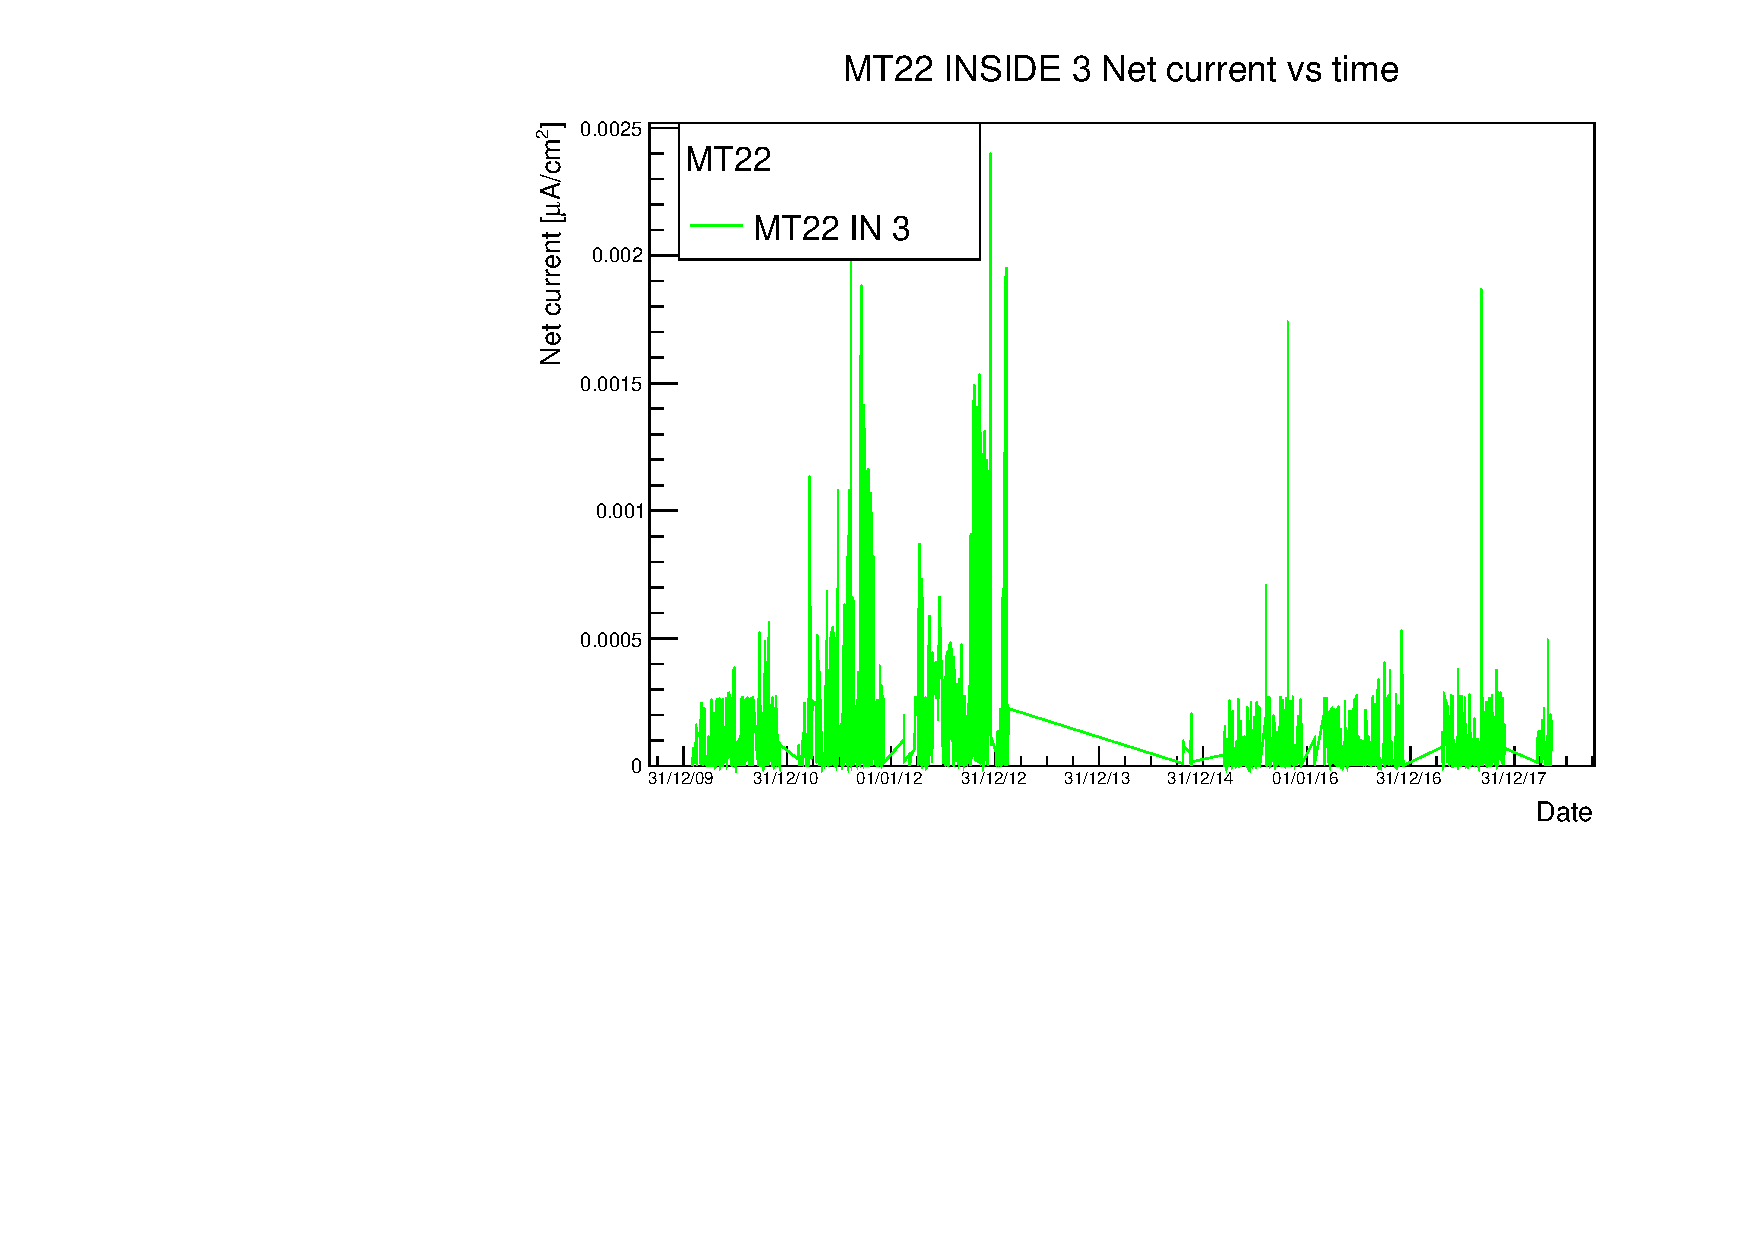
\includegraphics[width=0.95\linewidth]{Chapters/Performance/Figs/iNetFEERIC.pdf}
\caption{Net current as a function of time for the FEERIC-equipped RPC. The dark current is measured during cosmic runs, while the total current is measured during physics runs.}
\label{fig:FEERICiNet}
\end{center}
\end{figure}

The net current plot has been integrated over time in order to obtain the integrated charge growth over time.
% The integrated charge trend shows various slopes, spanning from constant behavior during shutdowns of LHC to steep growth during the highest luminosity periods.
The integrated charge can be estimated by integrating over time the currents of figure \ref{fig:iNet4Planes}. 
The result is shown in figure \ref{fig:ICharge4Planes}, where MT11, MT12, MT22 and MT21 are plotted (from top to bottom). 
The time interval with a constant charge corresponds to periods with no collisions at the LHC.
% The already noticed recovery effect, observed after the shutdowns while studying the dark current trends, can be observed in the integrated charge trend as well.
% After flat periods (i.e. periods with no irradiation of the chambers) the integrated charge growth starts slowly, increasing continuously.
% The detectors response to various levels of irradiation is not linear and depends on their previous status.
% This effect seems to suggest that the RPCs behavior depends on how much time they have at disposal to recover after a high irradiation period, as if the net current had some sort of inertia.
% Further monitoring and future specific tests might confirm such phenomenon.

\begin{figure}[!t]
\begin{center}
\includegraphics[width=0.95\linewidth]{Chapters/Performance/Figs/intCharge_vertical.pdf}
\caption{Integrated net charge for each RPC as a function of time. The 72 trends are divided by plane (from top to bottom MT11, MT12, MT21, MT22). For each plane the average plot is shown. Each point corresponds to a run.}
\label{fig:ICharge4Planes}
\end{center}
\end{figure}

% The comparison between different RPCs within the same plane highlights that their response to irradiation is neither constant in time nor constant between different detectors.
% Some detectors integrated charge overtakes on the one of other RPCs which present a much more stable behavior.
% While some RPCs present an integrated charge which is systematically higher than that of the rest of the RPCs of the plane, but the trend of the plot seems aligned with that of others, other RPCs present sudden variations of the trend slope.
% The RPCs which present sudden variations of the trend have to be monitored with attention as they might become the best candidates for a replacement.

The time series of MT12 outside 6 shows a sudden drop of the integrated charge. 
This is due to the fact that the RPC was replaced with a new one during the operations and the integrated charge has been therefore consistently reset to $0\mu C/cm^2$.

A detailed view of the FEERIC integrated charge is shown in figure \ref{fig:FEERICIntCharge}.
The shape reflects the lowering of the net current shown before (see Fig. \ref{fig:FEERICiNet}).
An integrated charge about $6$ times lower than the average for the plane has been collected by the RPC since the installation of the FEERIC electronics.

\begin{figure}[!t]
\begin{center}
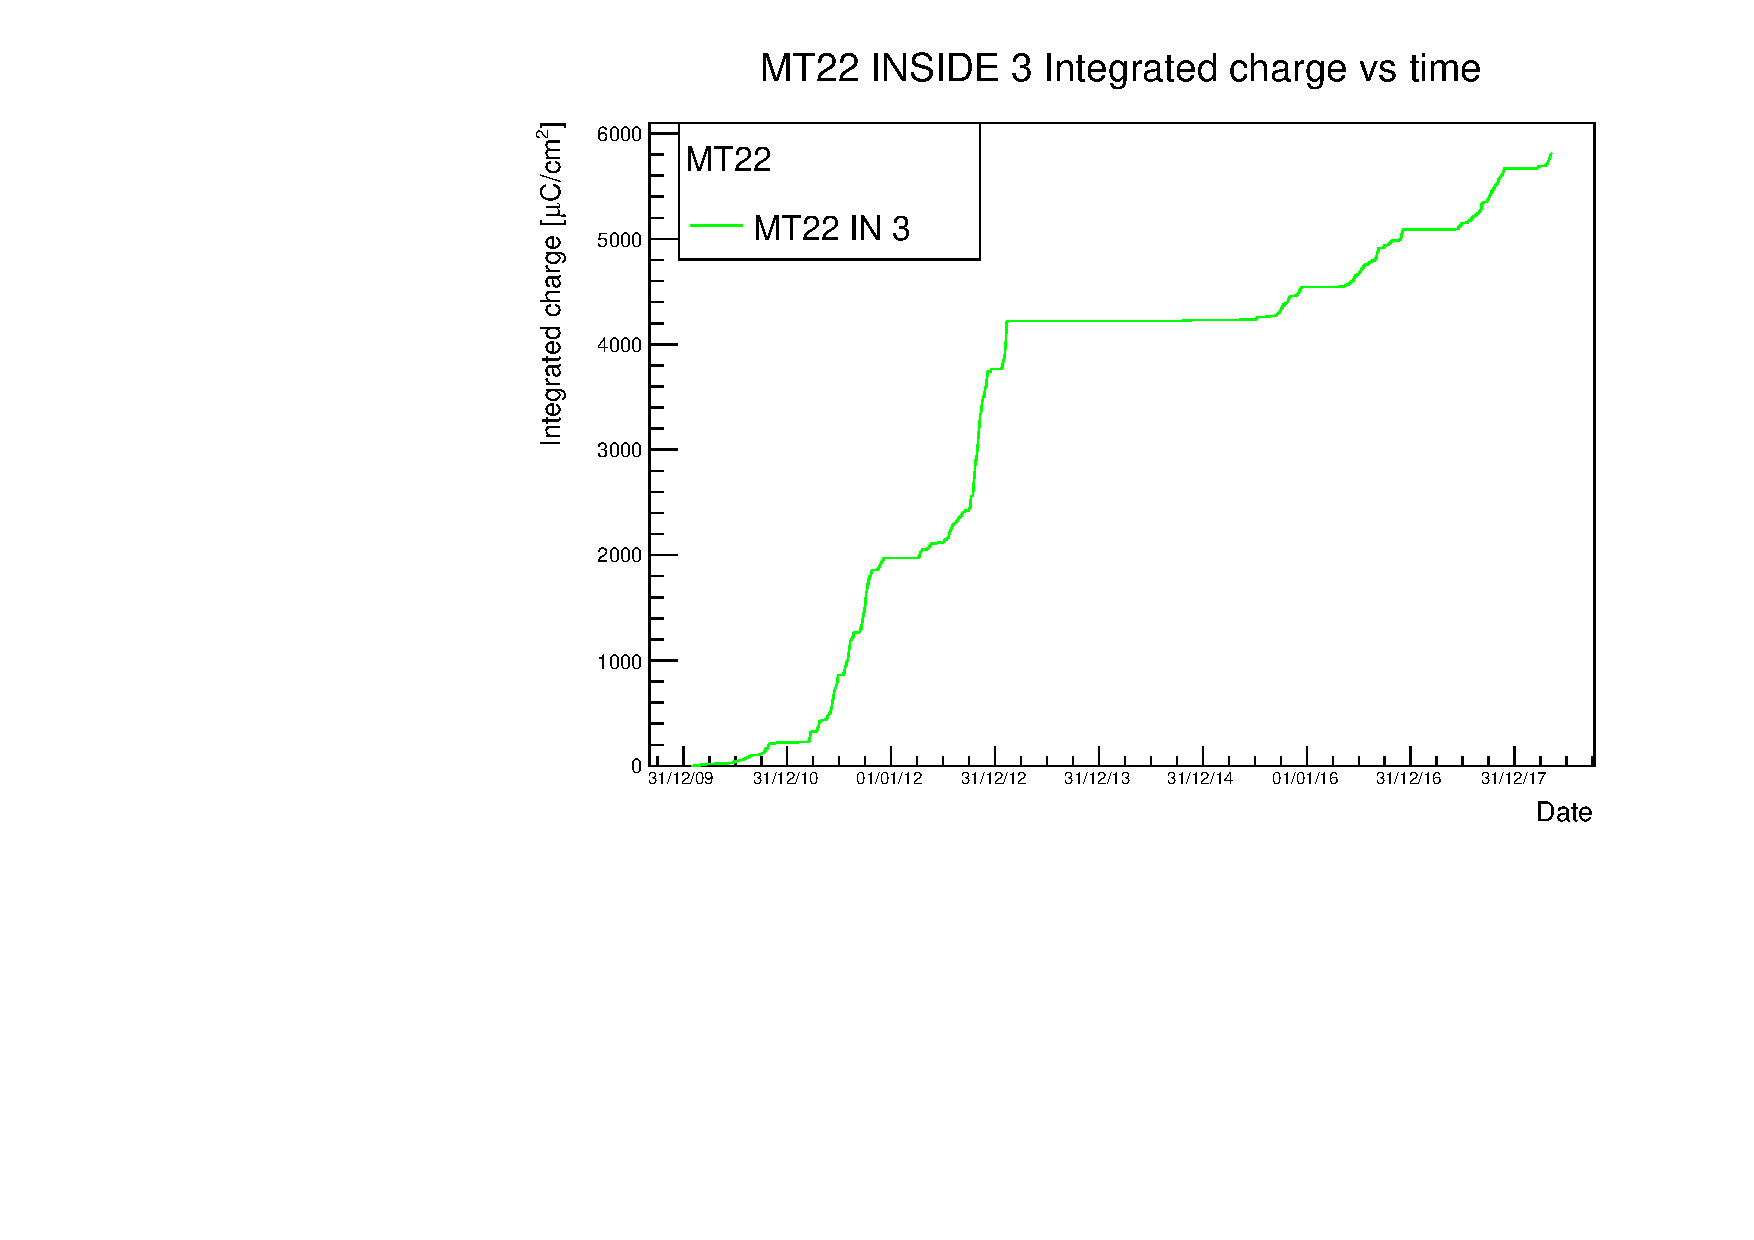
\includegraphics[width=0.95\linewidth]{Chapters/Performance/Figs/IntChargeFEERIC.pdf}
\caption{Integrated charge as a function of time for the FEERIC-equipped RPC. The $y$ value is the integral of net current shown in \ref{fig:FEERICiNet}.}
\label{fig:FEERICIntCharge}
\end{center}
\end{figure}

The results for the integrated charge show that, at the end of the 2017 run, the average integrated charge is about $8\ mC/cm^2$ (obtained by averaging the average values of the four planes), and the charge for the most exposed RPC is about $18\ mC/cm^2$. 
This is comfortably far from the limit of $50\ mC/cm^2$ reached in the ageing test. 
It has to be remarked that, when the charge is integrated without subtracting the dark current (i.e.assuming that $i_{dark}$ = $i_{noise}$) the results are larger by about a factor of two. 
Under this assumption, some RPCs may indeed be close to the end of their “certified lifetime”. 
Specific tests are needed to disentangle the ohmic component of the dark current. 
A possibility will be to measure the ohmic current at low voltage (where no amplification is possible in the gas, hence the noise-induced current is suppressed), and extrapolate it to the nominal voltage.

\subsection{Dark rate trend}
The dark rate trend is shown in figure \ref{fig:DarkRate4Planes}.
The information which can be obtained from this set of graphs is complementary to that of dark current one.
Observing an increase of the dark rate may be a symptom of aging.
In fact the dark rate is defined as the rate measured when no beam is present in the LHC.
The dark rate is then induced merely by environmental radioactive background or by spontaneous discharges in the gas gap.
For this reason, assuming the environmental background to be constant, any modification of the dark rate is induced by physical modifications of the inner surfaces or, in general, of the RPC health.

\begin{figure}[!t]
\begin{center}
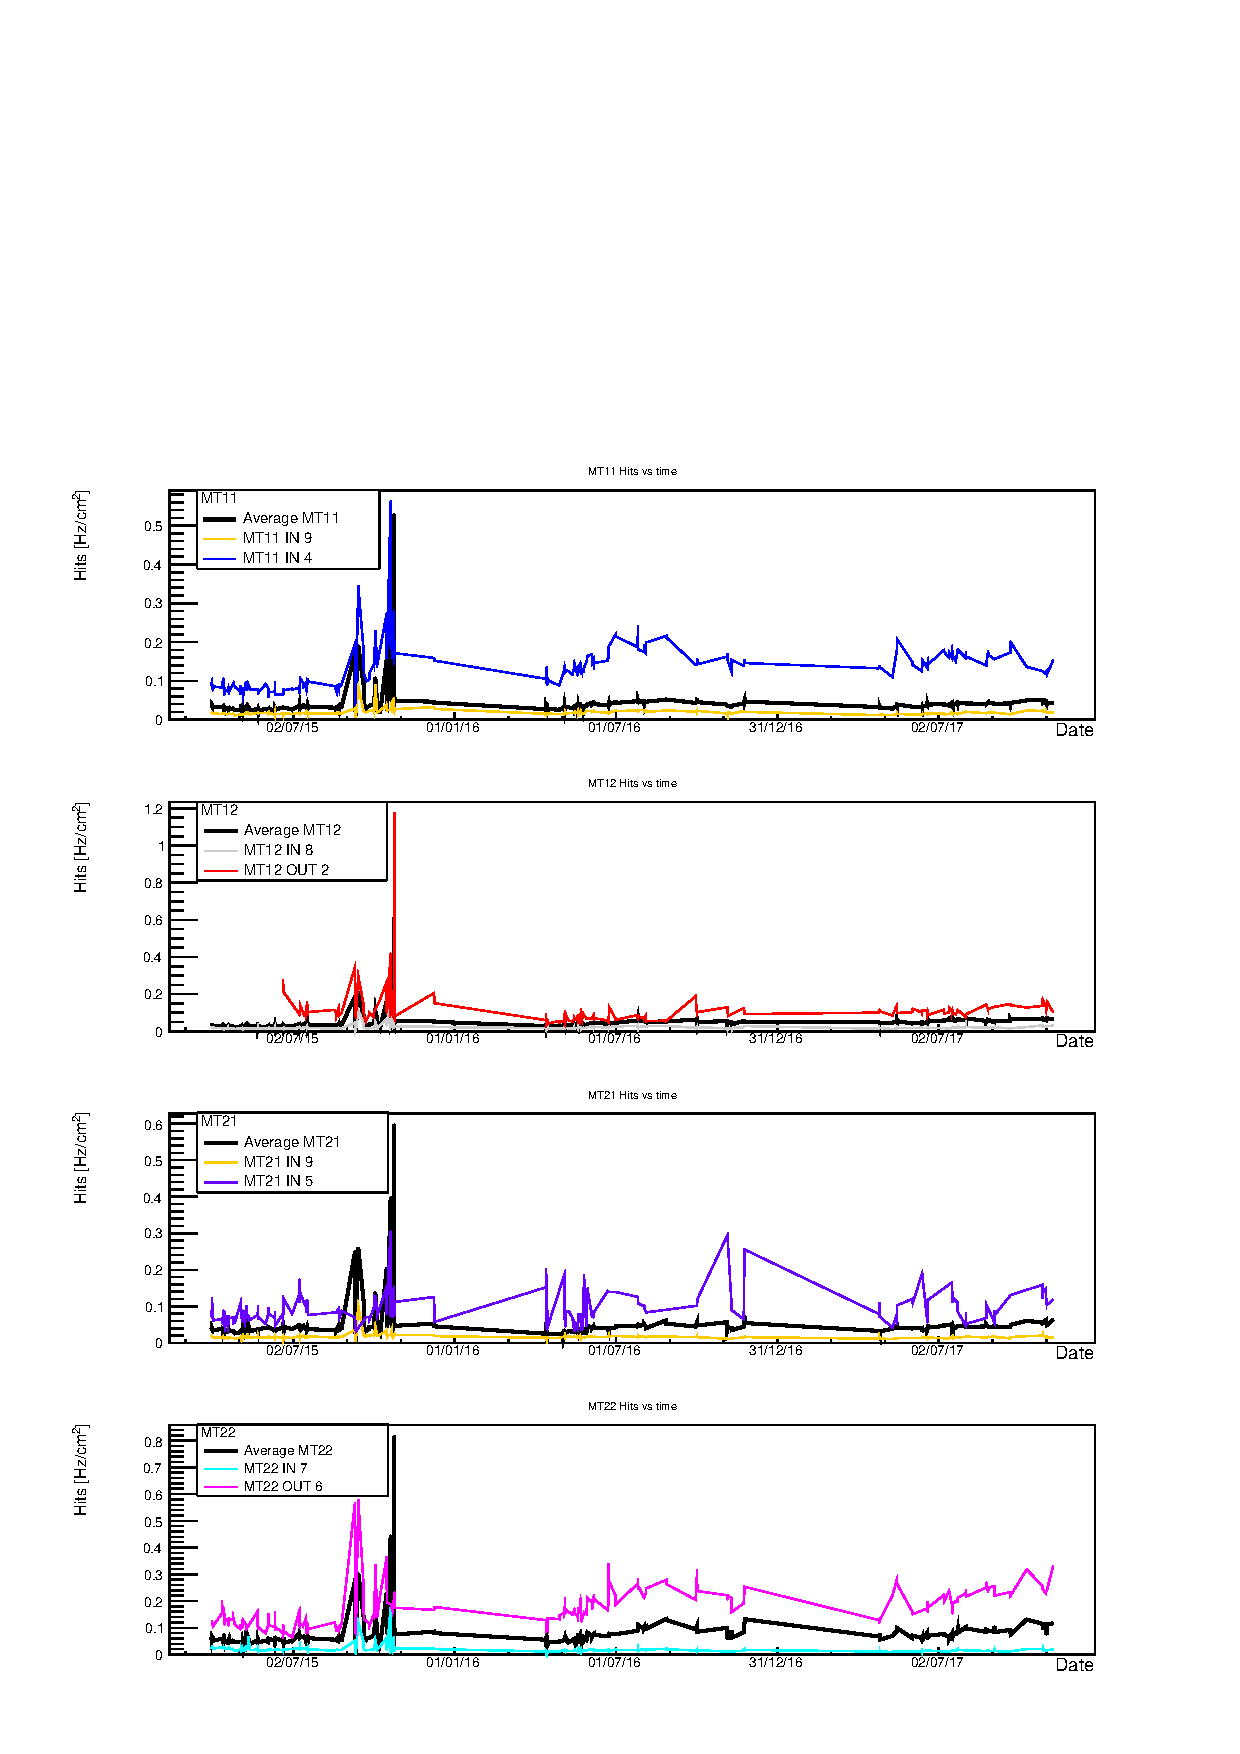
\includegraphics[width=0.95\linewidth]{Chapters/Performance/Figs/DarkRate.pdf}
\caption{Dark rates trends for each RPC over the whole operation period. The 72 trends are divided by plane (from top to bottom MT11, MT12, MT21, MT22). For each plane the average plot is shown. Each point corresponds to a run. The $y$ value is the average rate during a given cosmic run, while the $x$ value is the timestamp which corresponds to the end of run.}
\label{fig:DarkRate4Planes}
\end{center}
\end{figure}

In reality a variation of the environmental background should be taken into account.
In fact right after the beam operations some activation of material close to the MTR may be present.
For this reason a temporary increase of the dark rate is foreseen, even if the beam is not present anymore.
The signature one should look for is not a temporary increase of the dark rate, but a not complete recovery of the dark rate back to the level measured before a period with beam presence.

Analyzing the trends one can observe that some RPCs show a growth of the dark rate over the whole period of operation.
An average of $4-5$ RPCs per plane (not shown in the figure) present a large dark rate, well above average.
The chambers which show such behavior are the same that present an higher dark current with respect to the bulk of the RPCs.
It is worth mentioning that, even if some outliers are found, most of the RPCs are still operating at the original level of dark rate after around 8 years of continuous operation.
In that sense the dark rate trend is a good cross-check of the symptoms already detected with the dark current studies and the integrated charge ones.
The affected RPCs have to be monitored to check their efficiency and to constantly ensure that their effectiveness as detectors is not being affected by the increase of the dark rate.

The dark rate trend for FEERIC is shown in figure \ref{fig:FEERICDarkRate}.
% shows how most of the ADULT-equipped RPCs trends are lower than the trend of the FEERIC-equipped one.
The dark rate trend is compatible with the average trend for the plane.
% This aspect confirms that the chamber's efficiency is not modified by the lowering of the working point and the displacement of the amplification process to the electronics.

\begin{figure}[!t]
\begin{center}
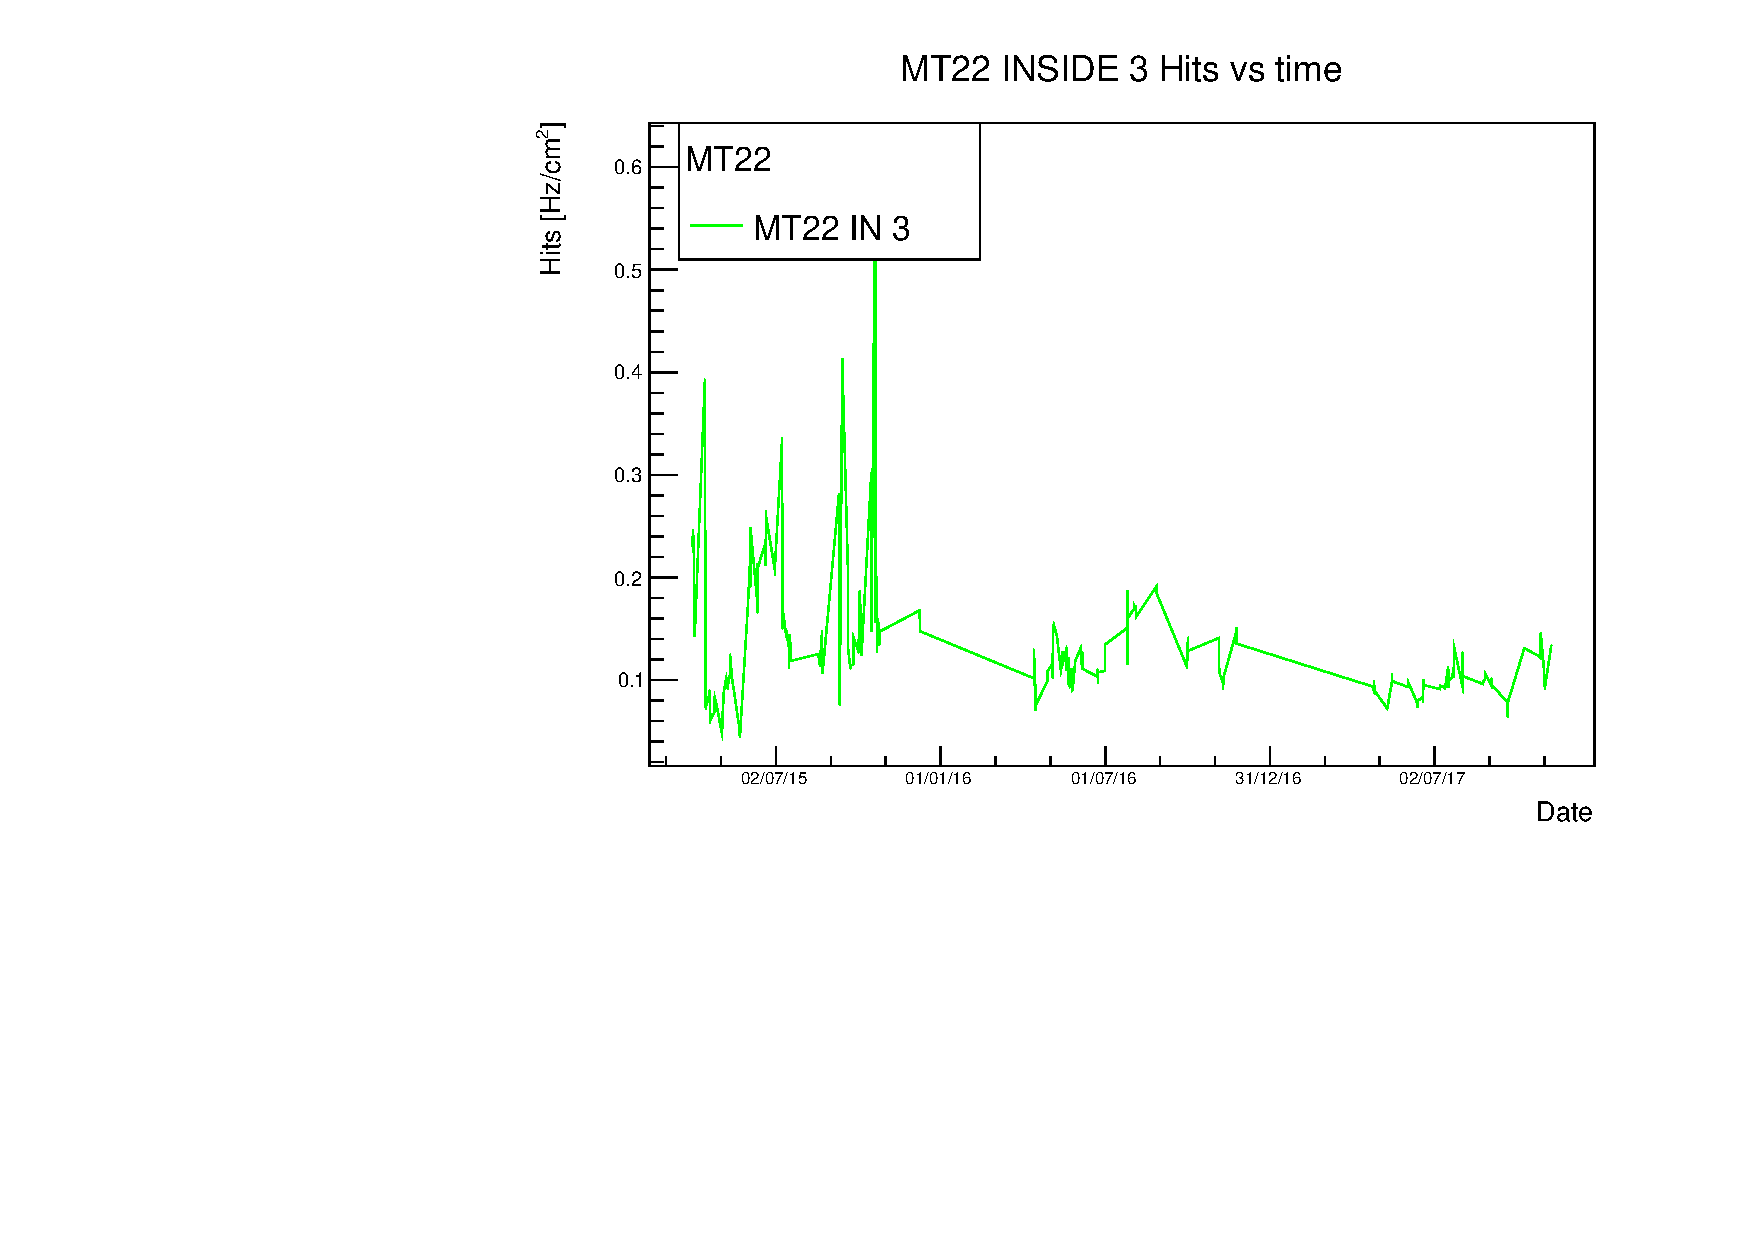
\includegraphics[width=0.95\linewidth]{Chapters/Performance/Figs/DarkRateFEERIC.pdf}
\caption{Dark rate trend for the FEERIC-equipped RPC. The $y$ value is the average rate measured during a given run, while the $x$ value is the timestamp which corresponds to the end of run.}
\label{fig:FEERICDarkRate}
\end{center}
\end{figure}

\subsection{Correlations between rates and net current}
The possibility to study correlations of different parameters was introduced with the new analysis framework.
The correlations are valuable tools to provide a deeper understanding of the RPC.
The correlation plot which allows to better understand the health of a detector is the one representing net current values correlated with measured rate.

The estimated net current of an RPC is expected to be proportional to the hit rate of the chamber itself.
This proportionality is related to the charge deposited in the detector per each hit.
The corresponding correlation can therefore easily highlight the presence of RPCs with abnormal discharge per hit.
The correlation of the net current as a function of the hit rate during periods with collisions is shown in figure \ref{fig:iNetvsRate4Planes}.
% Looking to the correlation plot, the slope shown by the bulk of points relative to a given RPC is correlated to the charge deposed in the detector per each hit.
% Fitting the correlation plot with a line can extract that value.
% This derived measurement is interesting, since can easily highlight RPCs with abnormal discharge per hit.
% Worth pointing out that this procedure won't highlight the presence of noisy channels which discharge easier, since such events would modify both terms of the ratio defining the slope of the graph.
% One can observe that the bulk of measurements has a transversal size which is neither negligible nor compatible with a straight line.
One can observe that for most of the measurements there is a strong correlation between the net current and the estimated rate. 
The correlation however is not perfect, and, for a given rate, a dispersion of the net currents can be observed.
% Such deviations can be due to different energies of the crossing particles as well as different crossing angles, resulting in different path length in the gas gap.
Such deviations can in principle be due to different energies of the crossing particles as well as different crossing angles, resulting in different path length in the gas gap, or to an intrinsically different response of different chambers.
They may also simply come from a bias in the calculation of the hit rate. 
This is calculated by summing up the rate of all strips, and no correction for the cluster size is possible. 
Such a bias depends on the segmentation of the read-out, hence it can be different for different RPCs.
% Deviations leading to this spread are related to different energies of the crossing particle and various crossing angles of the particle.
% A stronger (weaker) ionizing power and longer (shorter) path inside the gas gap work together to create deviations from the average behavior.

% The correlation plot of net current and rate with beam presence is shown in figure \ref{fig:iNetvsRate4Planes}.
% The behavior of the RPCs revealed by this correlation plot is aligned with previous measurements of other working parameters: while most of the chambers show a similar correlation between the two measurements, some of them clearly deviate from the bulk of points.
% In order to have a smaller dead time after a hit (the time required to recover the local HV drop) the charge released per hit should be kept as low as possible.
% A displacement the points to a zone representing lower charge deposed per hit is rarely (if not) expected, since the RPC health and status should worsen over time.
% Points showing a displacement in this direction are rare and not grouped in clusters.
% The absence of measurements clustering allows to suppose that the same causes of the bulk transversal spreading are responsible for these displacements.
% Displacements towards the zone of the plot representing a higher charge per hit are instead typical, since the conductivity of the gas gap can increase over time.
% In this case one can immediately note that such displaced points are grouped in clusters.
% Since each point represents one of the analyzed runs, the fact that in various runs a given RPC has shown a recurring higher charge per hit gives more significance to the measurement.

\begin{figure}[!t]
\begin{center}
\includegraphics[width=0.95\linewidth]{Chapters/Performance/Figs/iNet_vs_rate_vertical.pdf}
\caption{Correlation plot between net current and average rate within a given run. The 72 correlation plots are divided by plane (from top to bottom MT11, MT12, MT21, MT22). Each point corresponds to a run. The $y$ value is the average rate during a given cosmic run, while the $x$ value is the average net current value measured during the run.}
\label{fig:iNetvsRate4Planes}
\end{center}
\end{figure}

% As a side note, if we imagine to look at the correlation plot for a single RPC and to compute the distance between the extreme left and right points, we can take such value as an estimator of the variability of the rate hitting that RPC.
% An RPC which receives constantly a given rate will have a correlation plot with low span over rate axis, while an RPC with a rate which changes a lot (for example depending on the type of colliding system) will have a large span on the rates axis.
% Following this argument it is interesting how most part of the RPCs which show a derive to higher charge per hit are also the ones with the largest rate spans.
% This observation suggests that RPCs are affected by rates variations, more than from the integrated rate.
% More measurements could help better addressing this argument.
The FEERIC-equipped RPC, located in MT22, shows a systematically smaller charge per hit.
The slope of its correlation plot is much lower than that of the other RPCs of MT22 and results, as expected, in a lower deposed charge per hit.
% The transverse size of the distribution is smaller than that of ADULT RPCs.

\subsection{Chambers efficiency}
The new framework has been introduced for several reasons connected to the extension of the existing ALICE DCS Shuttle to more general use cases.
One of the features that will be used in the future is the possibility to add other values to perform additional correlations.
For example it is interesting to correlate aging effects to efficiency drops.
% Unfortunately the chambers efficiency is not yet published to the ALICE OCDB, hence this further development wasn't possible yet.
The chambers efficiency measurements are not yet integrated in the framework presented here.
It is however possible to show some efficiency studies to look for an efficiency modification which could be qualitatively correlated with some of the aging indicators already presented.
The efficiency trends from 2015 up to 2017 are shown in figures \ref{fig:MTR11efficiency}, \ref{fig:MTR12efficiency}, \ref{fig:MTR21efficiency} and \ref{fig:MTR22efficiency} for MT11, MT12, MT21 and MT22 respectively.

\begin{figure}[!ht]
\begin{center}
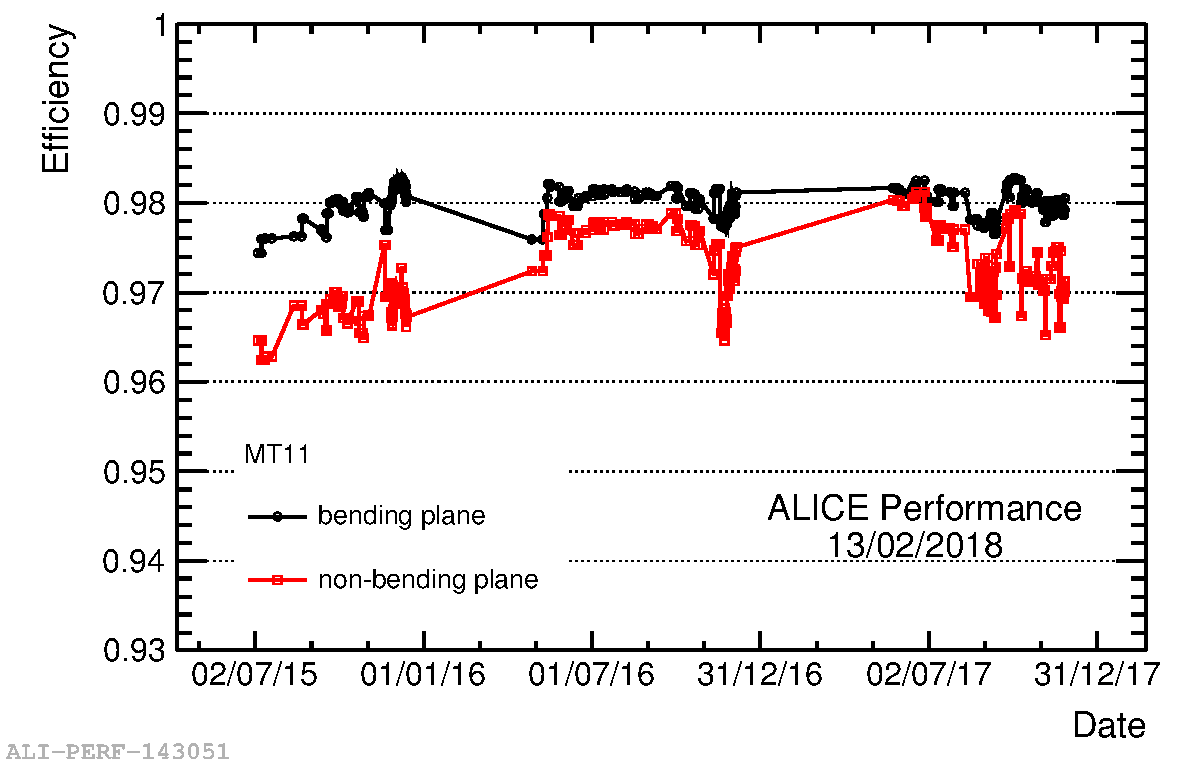
\includegraphics[width=0.8\linewidth]{Chapters/Performance/Figs/2018-Feb-16-effTrend_2015-2017_Ch11.pdf}
\caption{Average efficiency trend for MT11. Each point corresponds to a run. Bending and non bending planes are shown in black and red respectively.}
\label{fig:MTR11efficiency}
\end{center}
\end{figure}

\begin{figure}[!ht]
\begin{center}
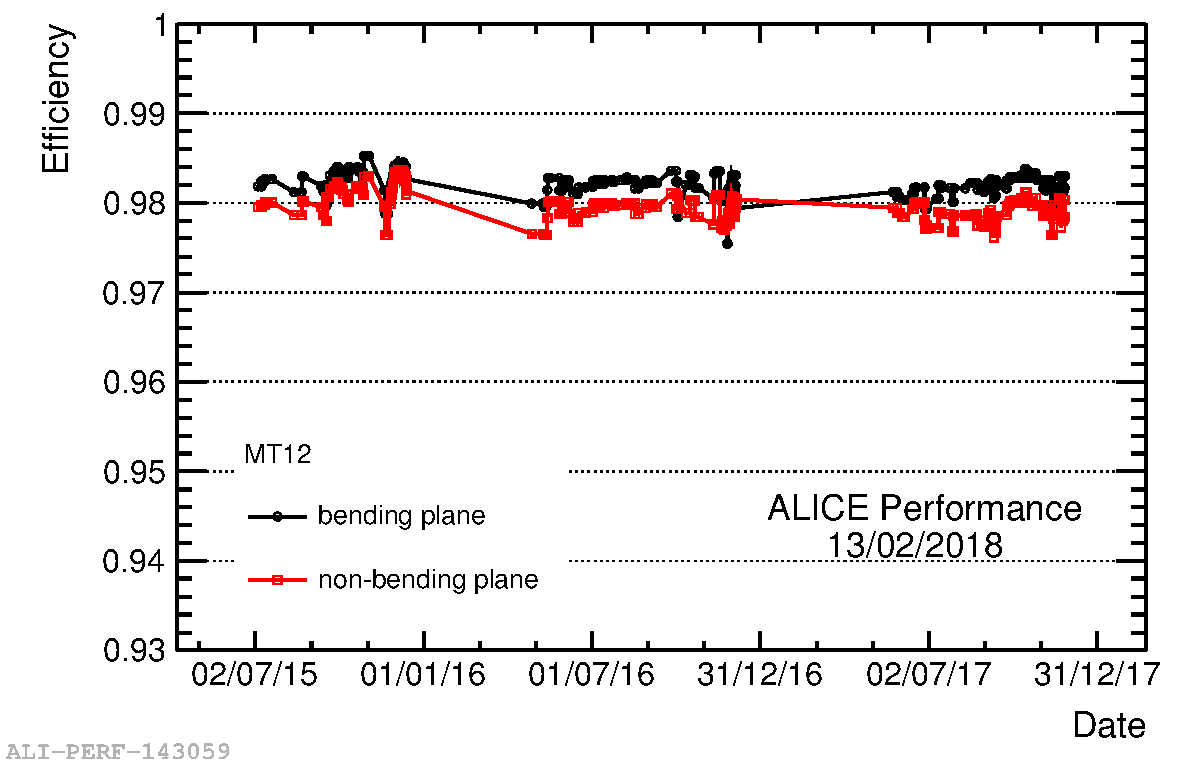
\includegraphics[width=0.8\linewidth]{Chapters/Performance/Figs/2018-Feb-16-effTrend_2015-2017_Ch12.pdf}
\caption{Average efficiency trend for MT12. Each point corresponds to a run. Bending and non bending planes are shown in black and red respectively.}
\label{fig:MTR12efficiency}
\end{center}
\end{figure}

\begin{figure}[!hb]
\begin{center}
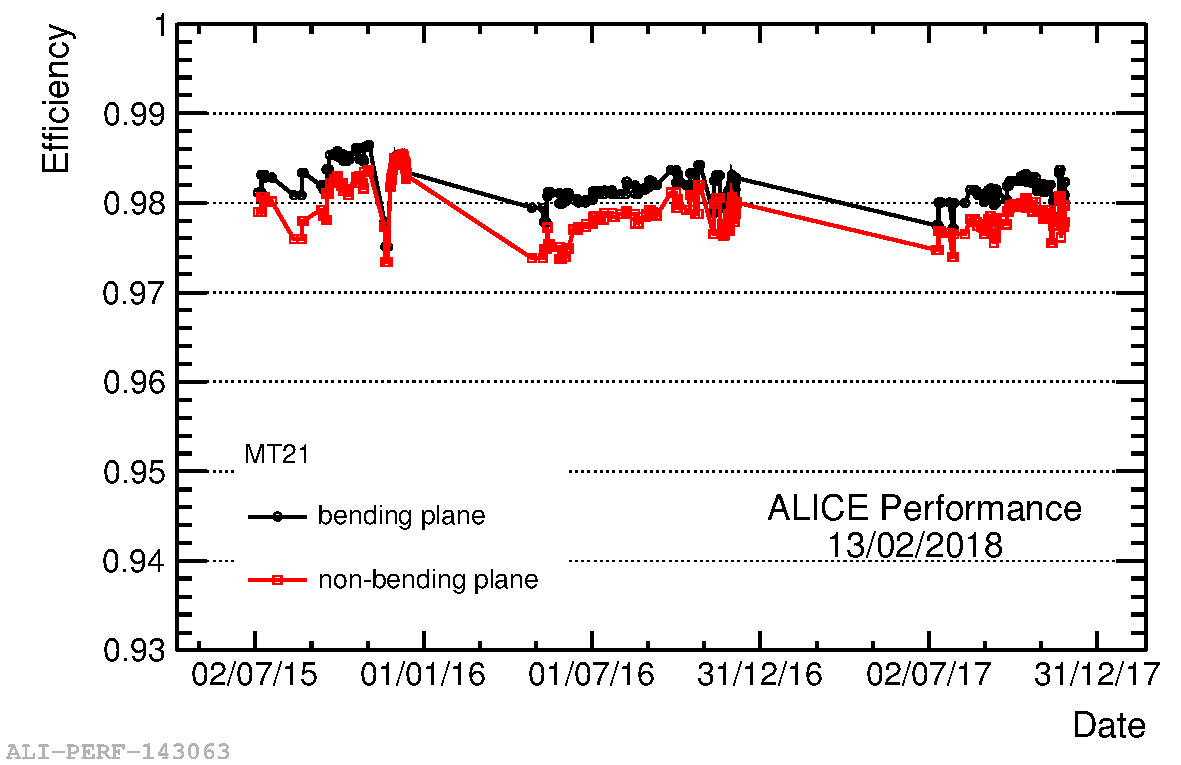
\includegraphics[width=0.8\linewidth]{Chapters/Performance/Figs/2018-Feb-16-effTrend_2015-2017_Ch13.pdf}
\caption{Average efficiency trend for MT21. Each point corresponds to a run. Bending and non bending planes are shown in black and red respectively.}
\label{fig:MTR21efficiency}
\end{center}
\end{figure}

\begin{figure}[!ht]
\begin{center}
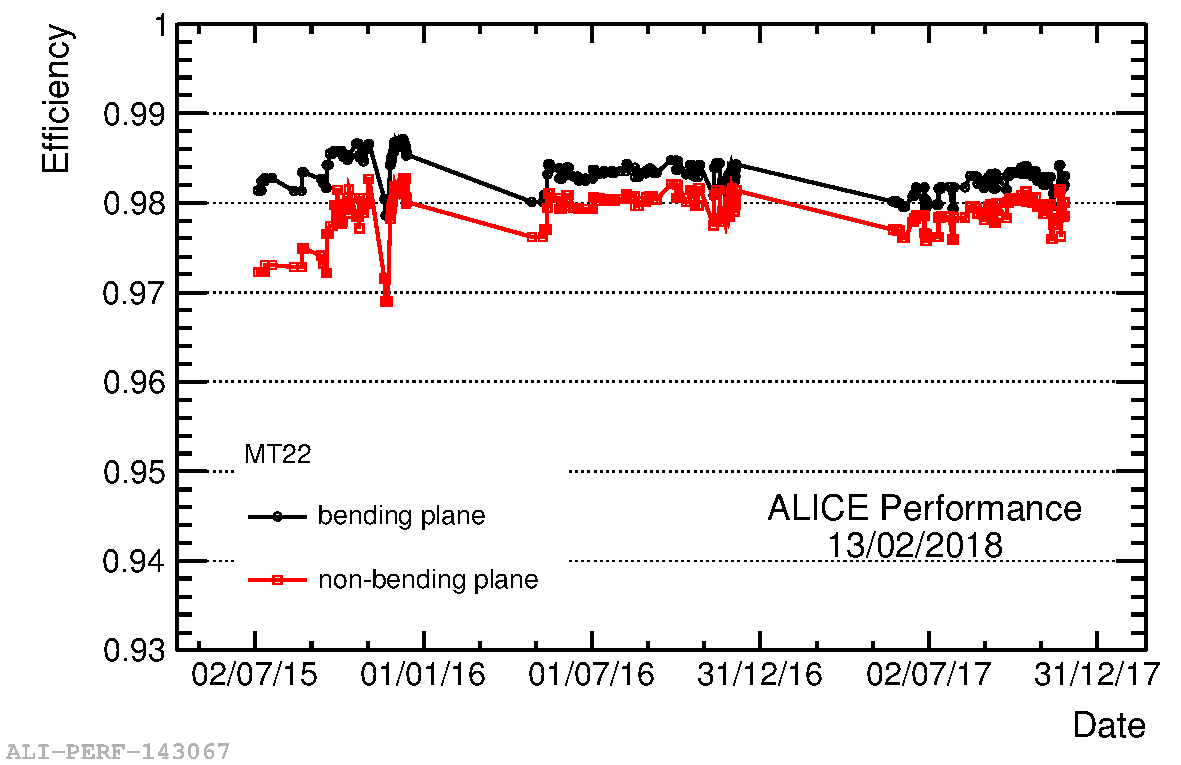
\includegraphics[width=0.8\linewidth]{Chapters/Performance/Figs/2018-Feb-16-effTrend_2015-2017_Ch14.pdf}
\caption{Average efficiency trend for MT22. Each point corresponds to a run. Bending and non bending planes are shown in black and red respectively.}
\label{fig:MTR22efficiency}
\end{center}
\end{figure}

\begin{figure}[!hb]
\begin{center}
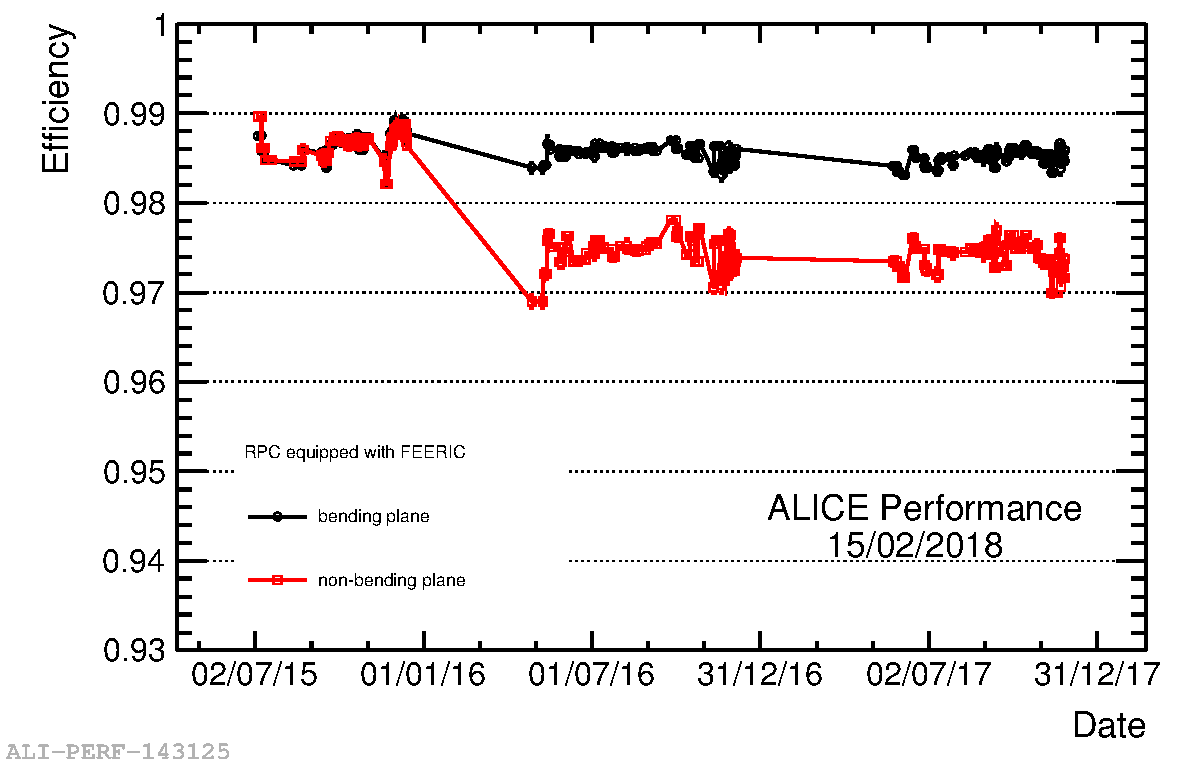
\includegraphics[width=0.8\linewidth]{Chapters/Performance/Figs/2018-Feb-16-effTrend_2015-2017_FEERIC.pdf}
\caption{Efficiency trend for the FEERIC-equipped RPC. Each point corresponds to a run. Bending and non bending planes are shown in black and red respectively.}
\label{fig:MTRFEERICefficiency}
\end{center}
\end{figure}

% Even if from the integrated charge and dark current evaluation, some aging effects are detected ($e.g.$ the integrated charge has grown faster during RUN2, the dark current seems to grow monotonically), the performance seems not to be affected by such effects.
The efficiency trend is measured as stable over the whole period and no worsening of the performance has been observed moving from the "relaxed" conditions of RUN1 to the RUN2 higher luminosity levels.
These arguments allow one to conclude that the RPCs of the ALICE muon trigger are performing at nominal efficiency, even if some aging effects are present and require continuous monitoring to detect possible variations.